\documentclass[type=bachelor,pifootnote]{thuthesis}
% 选项:
%   type=[bachelor|master|doctor|postdoctor], % 必选
%   secret,                                   % 可选
%   pifootnote,                               % 可选(建议打开)
%   openany|openright,                        % 可选,基本不用
%   arial,                                    % 可选,基本不用
%   arialtoc,                                 % 可选,基本不用
%   arialtitle                                % 可选,基本不用

% 所有其它可能用到的包都统一放到这里了,可以根据自己的实际添加或者删除。
\usepackage{thuthesis}
\usepackage{tikz}
\usepackage{pgfplots}
\usepackage{pgfplotstable}
\usepackage{bm}

% 定义所有的图片文件在 figures 子目录下
\graphicspath{{figures/}}

% 可以在这里修改配置文件中的定义。导言区可以使用中文。
% \def\myname{薛瑞尼}

\begin{document}

%%% 封面部分
\frontmatter
\thusetup{
  %******************************
  % 注意:
  %   1. 配置里面不要出现空行
  %   2. 不需要的配置信息可以删除
  %******************************
  %
  %=====
  % 秘级
  %=====
  secretlevel={秘密},
  secretyear={10},
  %
  %=========
  % 中文信息
  %=========
  ctitle={基于车路协同的车道汇合\\群决策问题研究},
  cdegree={工学硕士},
  cdepartment={~~自~动~化~系},
  cmajor={~~自~动~化},
  cauthor={~~陈~昊~楠},
  csupervisor={~~张~毅\hspace*{16pt}教~授},
  % cassosupervisor={陈文光教授}, % 副指导老师
  % ccosupervisor={某某某教授}, % 联合指导老师
  % 日期自动使用当前时间,若需指定按如下方式修改:
  % cdate={超新星纪元},
  %
  % 博士后专有部分
  cfirstdiscipline={计算机科学与技术},
  cseconddiscipline={系统结构},
  postdoctordate={2009年7月——2011年7月},
  id={编号}, % 可以留空: id={},
  udc={UDC}, % 可以留空
  catalognumber={分类号}, % 可以留空
  %
  %=========
  % 英文信息
  %=========
  etitle={An Introduction to \LaTeX{} Thesis Template of Tsinghua University v\version},
  % 这块比较复杂,需要分情况讨论:
  % 1. 学术型硕士
  %    edegree:必须为Master of Arts或Master of Science(注意大小写)
  %             “哲学、文学、历史学、法学、教育学、艺术学门类,公共管理学科
  %              填写Master of Arts,其它填写Master of Science”
  %    emajor:“获得一级学科授权的学科填写一级学科名称,其它填写二级学科名称”
  % 2. 专业型硕士
  %    edegree:“填写专业学位英文名称全称”
  %    emajor:“工程硕士填写工程领域,其它专业学位不填写此项”
  % 3. 学术型博士
  %    edegree:Doctor of Philosophy(注意大小写)
  %    emajor:“获得一级学科授权的学科填写一级学科名称,其它填写二级学科名称”
  % 4. 专业型博士
  %    edegree:“填写专业学位英文名称全称”
  %    emajor:不填写此项
  edegree={Doctor of Engineering},
  emajor={Computer Science and Technology},
  eauthor={Xue Ruini},
  esupervisor={Professor Zheng Weimin},
  eassosupervisor={Chen Wenguang},
  % 日期自动生成,若需指定按如下方式修改:
  % edate={December, 2005}
  %
  % 关键词用“英文逗号”分割
  ckeywords={\TeX, \LaTeX, CJK, 模板, 论文},
  ekeywords={\TeX, \LaTeX, CJK, template, thesis}
}

% 定义中英文摘要和关键字
\begin{cabstract}
  论文的摘要是对论文研究内容和成果的高度概括。摘要应对论文所研究的问题及其研究目
  的进行描述,对研究方法和过程进行简单介绍,对研究成果和所得结论进行概括。摘要应
  具有独立性和自明性,其内容应包含与论文全文同等量的主要信息。使读者即使不阅读全
  文,通过摘要就能了解论文的总体内容和主要成果。

  论文摘要的书写应力求精确、简明。切忌写成对论文书写内容进行提要的形式,尤其要避
  免“第 1 章……;第 2 章……;……”这种或类似的陈述方式。

  本文介绍清华大学论文模板 \thuthesis{} 的使用方法。本模板符合学校的本科、硕士、
  博士论文格式要求。

  本文的创新点主要有:
  \begin{itemize}
    \item 用例子来解释模板的使用方法;
    \item 用废话来填充无关紧要的部分;
    \item 一边学习摸索一边编写新代码。
  \end{itemize}

  关键词是为了文献标引工作、用以表示全文主要内容信息的单词或术语。关键词不超过 5
  个,每个关键词中间用分号分隔。(模板作者注:关键词分隔符不用考虑,模板会自动处
  理。英文关键词同理。)
\end{cabstract}

% 如果习惯关键字跟在摘要文字后面,可以用直接命令来设置,如下:
% \ckeywords{\TeX, \LaTeX, CJK, 模板, 论文}

\begin{eabstract}
   An abstract of a dissertation is a summary and extraction of research work
   and contributions. Included in an abstract should be description of research
   topic and research objective, brief introduction to methodology and research
   process, and summarization of conclusion and contributions of the
   research. An abstract should be characterized by independence and clarity and
   carry identical information with the dissertation. It should be such that the
   general idea and major contributions of the dissertation are conveyed without
   reading the dissertation.

   An abstract should be concise and to the point. It is a misunderstanding to
   make an abstract an outline of the dissertation and words ``the first
   chapter'', ``the second chapter'' and the like should be avoided in the
   abstract.

   Key words are terms used in a dissertation for indexing, reflecting core
   information of the dissertation. An abstract may contain a maximum of 5 key
   words, with semi-colons used in between to separate one another.
\end{eabstract}

% \ekeywords{\TeX, \LaTeX, CJK, template, thesis}

% 如果使用授权说明扫描页,将可选参数中指定为扫描得到的 PDF 文件名,例如:
% \makecover[scan-auth.pdf]
\makecover

%% 目录
\tableofcontents

%% 符号对照表
\begin{denotation}[3cm]
% \item[HPC] 高性能计算 (High Performance Computing)
% \item[cluster] 集群
% \item[Itanium] 安腾
% \item[SMP] 对称多处理
% \item[API] 应用程序编程接口
% \item[PI] 聚酰亚胺
% \item[MPI] 聚酰亚胺模型化合物,N-苯基邻苯酰亚胺
% \item[PBI] 聚苯并咪唑
% \item[MPBI] 聚苯并咪唑模型化合物,N-苯基苯并咪唑
% \item[PY] 聚吡咙
% \item[PMDA-BDA]	均苯四酸二酐与联苯四胺合成的聚吡咙薄膜
% \item[$\Delta G$] 活化自由能 (Activation Free Energy)
% \item[$\chi$] 传输系数 (Transmission Coefficient)
% \item[$E$] 能量
% \item[$m$] 质量
% \item[$c$] 光速
% \item[$P$] 概率
% \item[$T$] 时间
% \item[$v$] 速度
% \item[劝学] 君子曰:学不可以已。青,取之于蓝,而青于蓝;冰,水为之,而寒于水。木
%   直中绳。輮以为轮,其曲中规。虽有槁暴,不复挺者,輮使之然也。故木受绳则直,金就
%   砺则利,君子博学而日参省乎己,则知明而行无过矣。吾尝终日而思矣,不如须臾之所学
%   也;吾尝跂而望矣,不如登高之博见也。登高而招,臂非加长也,而见者远;顺风而呼,
%   声非加疾也,而闻者彰。假舆马者,非利足也,而致千里;假舟楫者,非能水也,而绝江
%   河,君子生非异也,善假于物也。积土成山,风雨兴焉;积水成渊,蛟龙生焉;积善成德,
%   而神明自得,圣心备焉。故不积跬步,无以至千里;不积小流,无以成江海。骐骥一跃,
%   不能十步;驽马十驾,功在不舍。锲而舍之,朽木不折;锲而不舍,金石可镂。蚓无爪牙
%   之利,筋骨之强,上食埃土,下饮黄泉,用心一也。蟹六跪而二螯,非蛇鳝之穴无可寄托
%   者,用心躁也。—— 荀况
\item[$L$] 控制区长度
\item[$S$] 交汇区长度
\item[$p_i$] 位移量
\item[$v_i$] 速度
\item[$\bm{x}_i$] 状态量
\item[$u_i$] 控制量,加速度
\item[$\mathcal{P}$] 可行位移集
\item[$\mathcal{V}$] 可行速度集
\item[$\mathcal{X}$] 可行状态量集
\item[$\mathcal{U}$] 可行控制量集,可行加速度集
\item[$\mathcal{N}(t)$] $t$时刻所有车辆编号集
\item[$\mathcal{L}_i$] 与$i$同一车道的车辆编号集
\item[$\mathcal{C}_i$] 与$i$不同车道的车辆编号集
\item[$t_i^0$] 进入控制区时间
\item[$t_i^\mathrm{m}$] 进入交汇区时间
\item[$t_i^\mathrm{f}$] 离开交汇区时间
\item[$\Gamma$] 可能碰撞集
\item[$v_\mathrm{d}$] 期望速度
\item[$J(\bm{u})$] 目标函数
\item[$H$] 哈密尔顿函数
\end{denotation}



%%% 正文部分
\mainmatter
\chapter{引言}
\label{cha:intro_old}

这是 \thuthesis{} 的示例文档,基本上覆盖了模板中所有格式的设置。建议大家在使用模
板之前,除了阅读《\thuthesis{}用户手册》,这个示例文档也最好能看一看。

小老鼠偷吃热凉粉;短长虫环绕矮高粱\footnote{韩愈(768-824),字退之,河南河阳(
  今河南孟县)人,自称郡望昌黎,世称韩昌黎。幼孤贫刻苦好学,德宗贞元八年进士。曾
  任监察御史,因上疏请免关中赋役,贬为阳山县令。后随宰相裴度平定淮西迁刑部侍郎,
  又因上表谏迎佛骨,贬潮州刺史。做过吏部侍郎,死谥文公,故世称韩吏部、韩文公。是
  唐代古文运动领袖,与柳宗元合称韩柳。诗力求险怪新奇,雄浑重气势。}。


\section{研究背景}
封面的例子请参看 cover.tex。主要符号表参看 denation.tex,附录和个人简历分别参看 appendix01.tex
和 resume.tex。里面的命令都很直观,一看即会\footnote{你说还是看不懂?怎么会呢?}。

\section{字体命令}
\label{sec:first}

苏轼(1037-1101),北宋文学家、书画家。字子瞻,号东坡居士,眉州眉山(今属四川)人
。苏洵子。嘉佑进士。神宗时曾任祠部员外郎,因反对王安石新法而求外职,任杭州通判,
知密州、徐州、湖州。后以作诗“谤讪朝廷”罪贬黄州。哲宗时任翰林学士,曾出知杭州、
颖州等,官至礼部尚书。后又贬谪惠州、儋州。北还后第二年病死常州。南宋时追谥文忠。
与父洵弟辙,合称“三苏”。在政治上属于旧党,但也有改革弊政的要求。其文汪洋恣肆,
明白畅达,为“唐宋八大家”之一。  其诗清新豪健,善用夸张比喻,在艺术表现方面独具
风格。少数诗篇也能反映民间疾苦,指责统治者的奢侈骄纵。词开豪放一派,对后代很有影
响。《念奴娇·赤壁怀古》、《水调歌头·丙辰中秋》传诵甚广。

{\kaishu 坡仙擅长行书、楷书,取法李邕、徐浩、颜真卿、杨凝式,而能自创新意。用笔丰腴
  跌宕,有天真烂漫之趣。与蔡襄、黄庭坚、米芾并称“宋四家”。能画竹,学文同,也喜
  作枯木怪石。论画主张“神似”,认为“论画以形似,见与儿童邻”;高度评价“诗中有
  画,画中有诗”的艺术造诣。诗文有《东坡七集》等。存世书迹有《答谢民师论文帖》、
  《祭黄几道文》、《前赤壁赋》、《黄州寒食诗帖》等。  画迹有《枯木怪石图》、《
  竹石图》等。}

{\fangsong 易与天地准,故能弥纶天地之道。仰以观於天文,俯以察於地理,是故知幽明之故。原
  始反终,故知死生之说。精气为物,游魂为变,是故知鬼神之情状。与天地相似,故不违。
  知周乎万物,而道济天下,故不过。旁行而不流,乐天知命,故不忧。安土敦乎仁,故
  能爱。范围天地之化而不过,曲成万物而不遗,通乎昼夜之道而知,故神无方而易无体。}

% 非本科生一般用不到幼圆与隶书字体。需要的同学请查看 ctex 文档。
{\ifcsname youyuan\endcsname\youyuan\else[无 \cs{youyuan} 字体。]\fi 有天地,然后
  万物生焉。盈天地之间者,唯万物,故受之以屯;屯者盈也,屯者物之始生也。物生必蒙,
  故受之以蒙;蒙者蒙也,物之穉也。物穉不可不养也,故受之以需;需者饮食之道也。饮
  食必有讼,故受之以讼。讼必有众起,故受之以师;师者众也。众必有所比,故受之以比;
  比者比也。比必有所畜也,故受之以小畜。物畜然后有礼,故受之以履。}

{\heiti 履而泰,然后安,故受之以泰;泰者通也。物不可以终通,故受之以否。物不可以终
  否,故受之以同人。与人同者,物必归焉,故受之以大有。有大者不可以盈,故受之以谦。
  有大而能谦,必豫,故受之以豫。豫必有随,故受之以随。以喜随人者,必有事,故受
  之以蛊;蛊者事也。}

{\ifcsname lishu\endcsname\lishu\else[无 \cs{lishu} 字体。]\fi 有事而后可大,故受
  之以临;临者大也。物大然后可观,故受之以观。可观而后有所合,故受之以噬嗑;嗑者
  合也。物不可以苟合而已,故受之以贲;贲者饰也。致饰然后亨,则尽矣,故受之以剥;
  剥者剥也。物不可以终尽,剥穷上反下,故受之以复。复则不妄矣,故受之以无妄。}

{\songti 有无妄然后可畜,故受之以大畜。物畜然后可养,故受之以颐;颐者养也。不养则不
  可动,故受之以大过。物不可以终过,故受之以坎;坎者陷也。陷必有所丽,故受之以
  离;离者丽也。}

\section{表格样本}
\label{chap1:sample:table}

\subsection{基本表格}
\label{sec:basictable}

模板中关于表格的宏包有三个: \pkg{booktabs}、\pkg{array} 和
\pkg{longtabular},命令有一个 \cs{hlinewd}。三线表可以用 \pkg{booktabs}
提供的 \cs{toprule}、\cs{midrule} 和 \cs{bottomrule}。它们与
\pkg{longtable} 能很好的配合使用。如果表格比较简单的话可以直接用命令
\cs{hlinewd}\marg{width} 控制。
\begin{table}[htb]
  \centering
  \begin{minipage}[t]{0.8\linewidth} % 如果想在表格中使用脚注,minipage是个不错的办法
  \caption[模板文件]{模板文件。如果表格的标题很长,那么在表格索引中就会很不美
    观,所以要像 chapter 那样在前面用中括号写一个简短的标题。这个标题会出现在索
    引中。}
  \label{tab:template-files}
    \begin{tabularx}{\linewidth}{lX}
      \toprule[1.5pt]
      {\heiti 文件名} & {\heiti 描述} \\\midrule[1pt]
      thuthesis.ins & \LaTeX{} 安装文件,\textsc{DocStrip}\footnote{表格中的脚注} \\
      thuthesis.dtx & 所有的一切都在这里面\footnote{再来一个}。\\
      thuthesis.cls & 模板类文件。\\
      thuthesis.cfg & 模板配置文。cls 和 cfg 由前两个文件生成。\\
      thuthesis.bst    & 参考文献 BIB\TeX\ 样式文件。\\
      thuthesis.sty   & 常用的包和命令写在这里,减轻主文件的负担。\\
      \bottomrule[1.5pt]
    \end{tabularx}
  \end{minipage}
\end{table}

首先来看一个最简单的表格。表 \ref{tab:template-files} 列举了本模板主要文件及其功
能。请大家注意三线表中各条线对应的命令。这个例子还展示了如何在表格中正确使用脚注。
由于 \LaTeX{} 本身不支持在表格中使用 \cs{footnote},所以我们不得不将表格放在
小页中,而且最好将表格的宽度设置为小页的宽度,这样脚注看起来才更美观。

\subsection{复杂表格}
\label{sec:complicatedtable}

我们经常会在表格下方标注数据来源,或者对表格里面的条目进行解释。前面的脚注是一种
不错的方法,如果不喜欢脚注,可以在表格后面写注释,比如表~\ref{tab:tabexamp1}。
\begin{table}[htbp]
  \centering
  \caption{复杂表格示例 1}
  \label{tab:tabexamp1}
  \begin{minipage}[t]{0.8\textwidth}
    \begin{tabularx}{\linewidth}{|l|X|X|X|X|}
      \hline
 \multirow{2}*{\diagbox[width=5em]{x}{y}} & \multicolumn{2}{c|}{First Half} & \multicolumn{2}{c|}{Second Half}\\\cline{2-5}
      & 1st Qtr &2nd Qtr&3rd Qtr&4th Qtr \\ \hline
      East$^{*}$ &   20.4&   27.4&   90&     20.4 \\
      West$^{**}$ &   30.6 &   38.6 &   34.6 &  31.6 \\ \hline
    \end{tabularx}\\[2pt]
    \footnotesize 注:数据来源《\thuthesis{} 使用手册》。\\
    *:东部\\
    **:西部
  \end{minipage}
\end{table}

此外,表~\ref{tab:tabexamp1} 同时还演示了另外两个功能:1)通过 \pkg{tabularx} 的
 \texttt{|X|} 扩展实现表格自动放大;2)通过命令 \cs{diagbox} 在表头部分
插入反斜线。

为了使我们的例子更接近实际情况,我会在必要的时候插入一些“无关”文字,以免太多图
表同时出现,导致排版效果不太理想。第一个出场的当然是我的最爱:风流潇洒、骏马绝尘、
健笔凌云的{\heiti 李太白}了。

李白,字太白,陇西成纪人。凉武昭王暠九世孙。或曰山东人,或曰蜀人。白少有逸才,志
气宏放,飘然有超世之心。初隐岷山,益州长史苏颋见而异之,曰:“是子天才英特,可比
相如。”天宝初,至长安,往见贺知章。知章见其文,叹曰:“子谪仙人也。”言于明皇,
召见金銮殿,奏颂一篇。帝赐食,亲为调羹,有诏供奉翰林。白犹与酒徒饮于市,帝坐沉香
亭子,意有所感,欲得白为乐章,召入,而白已醉。左右以水颒面,稍解,援笔成文,婉丽
精切。帝爱其才,数宴见。白常侍帝,醉,使高力士脱靴。力士素贵,耻之,摘其诗以激杨
贵妃。帝欲官白,妃辄沮止。白自知不为亲近所容,恳求还山。帝赐金放还。乃浪迹江湖,
终日沉饮。永王璘都督江陵,辟为僚佐。璘谋乱,兵败,白坐长流夜郎,会赦得还。族人阳
冰为当涂令,白往依之。代宗立,以左拾遗召,而白已卒。文宗时,诏以白歌诗、裴旻剑舞、
张旭草书为三绝云。集三十卷。今编诗二十五卷。\hfill —— 《全唐诗》诗人小传

浮动体的并排放置一般有两种情况:1)二者没有关系,为两个独立的浮动体;2)二者隶属
于同一个浮动体。对表格来说并排表格既可以像图~\ref{tab:parallel1}、图~\ref{tab:parallel2} 
使用小页环境,也可以如图~\ref{tab:subtable} 使用子表格来做。图的例子参见第~\ref{sec:multifig} 节。

\begin{table}[htbp]
\noindent\begin{minipage}{0.5\textwidth}
\centering
\caption{第一个并排子表格}
\label{tab:parallel1}
\begin{tabular}{p{2cm}p{2cm}}
\toprule[1.5pt]
111 & 222 \\\midrule[1pt]
222 & 333 \\\bottomrule[1.5pt]
\end{tabular}
\end{minipage}%
\begin{minipage}{0.5\textwidth}
\centering
\caption{第二个并排子表格}
\label{tab:parallel2}
\begin{tabular}{p{2cm}p{2cm}}
\toprule[1.5pt]
111 & 222 \\\midrule[1pt]
222 & 333 \\\bottomrule[1.5pt]
\end{tabular}
\end{minipage}
\end{table}

然后就是忧国忧民,诗家楷模杜工部了。杜甫,字子美,其先襄阳人,曾祖依艺为巩令,因
居巩。甫天宝初应进士,不第。后献《三大礼赋》,明皇奇之,召试文章,授京兆府兵曹参
军。安禄山陷京师,肃宗即位灵武,甫自贼中遁赴行在,拜左拾遗。以论救房琯,出为华州
司功参军。关辅饥乱,寓居同州同谷县,身自负薪采梠,餔糒不给。久之,召补京兆府功曹,
道阻不赴。严武镇成都,奏为参谋、检校工部员外郎,赐绯。武与甫世旧,待遇甚厚。乃于
成都浣花里种竹植树,枕江结庐,纵酒啸歌其中。武卒,甫无所依,乃之东蜀就高適。既至
而適卒。是岁,蜀帅相攻杀,蜀大扰。甫携家避乱荆楚,扁舟下峡,未维舟而江陵亦乱。乃
溯沿湘流,游衡山,寓居耒阳。卒年五十九。元和中,归葬偃师首阳山,元稹志其墓。天宝
间,甫与李白齐名,时称李杜。然元稹之言曰:“李白壮浪纵恣,摆去拘束,诚亦差肩子美
矣。至若铺陈终始,排比声韵,大或千言,次犹数百,词气豪迈,而风调清深,属对律切,
而脱弃凡近,则李尚不能历其藩翰,况堂奥乎。”白居易亦云:“杜诗贯穿古今,  尽工尽
善,殆过于李。”元、白之论如此。盖其出处劳佚,喜乐悲愤,好贤恶恶,一见之于诗。而
又以忠君忧国、伤时念乱为本旨。读其诗可以知其世,故当时谓之“诗史”。旧集诗文共六
十卷,今编诗十九卷。

\begin{table}[htbp]
\centering
\caption{并排子表格}
\label{tab:subtable}
\subcaptionbox{第一个子表格}
{
\begin{tabular}{p{2cm}p{2cm}}
\toprule[1.5pt]
111 & 222 \\\midrule[1pt]
222 & 333 \\\bottomrule[1.5pt]
\end{tabular}
}
\hskip2cm
\subcaptionbox{第二个子表格}
{
\begin{tabular}{p{2cm}p{2cm}}
\toprule[1.5pt]
111 & 222 \\\midrule[1pt]
222 & 333 \\\bottomrule[1.5pt]
\end{tabular}
}
\end{table}

不可否认 \LaTeX{} 的表格功能没有想象中的那么强大,不过只要足够认真,足够细致,
同样可以排出来非常复杂非常漂亮的表格。请参看表~\ref{tab:tabexamp2}。
\begin{table}[htbp]
  \centering\dawu[1.3]
  \caption{复杂表格示例 2}
  \label{tab:tabexamp2}
  \begin{tabular}[c]{|m{1.5cm}|c|c|c|c|c|c|}\hline
    \multicolumn{2}{|c|}{Network Topology} & \# of nodes & 
    \multicolumn{3}{c|}{\# of clients} & Server \\\hline
    GT-ITM & Waxman Transit-Stub & 600 &
    \multirow{2}{2em}{2\%}& 
    \multirow{2}{2em}{10\%}& 
    \multirow{2}{2em}{50\%}& 
    \multirow{2}{1.2in}{Max. Connectivity}\\\cline{1-3}
    \multicolumn{2}{|c|}{Inet-2.1} & 6000 & & & &\\\hline
    \multirow{2}{1.5cm}{Xue} & Rui  & Ni &\multicolumn{4}{c|}{\multirow{2}*{\thuthesis}}\\\cline{2-3}
    & \multicolumn{2}{c|}{ABCDEF} &\multicolumn{4}{c|}{} \\\hline
\end{tabular}
\end{table}

最后就是清新飘逸、文约意赅、空谷绝响的王大侠了。王维,字摩诘,河东人。工书画,与
弟缙俱有俊才。开元九年,进士擢第,调太乐丞。坐累为济州司仓参军,历右拾遗、监察御
史、左补阙、库部郎中,拜吏部郎中。天宝末,为给事中。安禄山陷两都,维为贼所得,服
药阳喑,拘于菩提寺。禄山宴凝碧池,维潜赋诗悲悼,闻于行在。贼平,陷贼官三等定罪,
特原之,责授太子中允,迁中庶子、中书舍人。复拜给事中,转尚书右丞。维以诗名盛于开
元、天宝间,宁薛诸王驸马豪贵之门,无不拂席迎之。得宋之问辋川别墅,山水绝胜,与道
友裴迪,浮舟往来,弹琴赋诗,啸咏终日。笃于奉佛,晚年长斋禅诵。一日,忽索笔作书
数纸,别弟缙及平生亲故,舍笔而卒。赠秘书监。宝应中,代宗问缙:“朕常于诸王坐闻维
乐章,今存几何?”缙集诗六卷,文四卷,表上之。敕答云,卿伯氏位列先朝,名高希代。
抗行周雅,长揖楚辞。诗家者流,时论归美。克成编录,叹息良深。殷璠谓维诗词秀调雅,
意新理惬。在泉成珠,著壁成绘。苏轼亦云:“维诗中有画,画中有诗也。”今编诗四卷。

要想用好论文模板还是得提前学习一些 \TeX/\LaTeX{}的相关知识,具备一些基本能力,掌
握一些常见技巧,否则一旦遇到问题还真是比较麻烦。我们见过很多这样的同学,一直以来
都是使用 Word 等字处理工具,以为 \LaTeX{}模板的用法也应该类似,所以就沿袭同样的思
路来对待这种所见非所得的排版工具,结果被折腾的焦头烂额,疲惫不堪。

如果您要排版的表格长度超过一页,那么推荐使用 \pkg{longtable} 或者 \pkg{supertabular}
宏包,模板对 \pkg{longtable} 进行了相应的设置,所以用起来可能简单一些。
表~\ref{tab:performance} 就是 \pkg{longtable} 的简单示例。
\begin{longtable}[c]{c*{6}{r}}
\caption{实验数据}\label{tab:performance}\\
\toprule[1.5pt]
 测试程序 & \multicolumn{1}{c}{正常运行} & \multicolumn{1}{c}{同步} & \multicolumn{1}{c}{检查点} & \multicolumn{1}{c}{卷回恢复}
& \multicolumn{1}{c}{进程迁移} & \multicolumn{1}{c}{检查点} \\
& \multicolumn{1}{c}{时间 (s)}& \multicolumn{1}{c}{时间 (s)}&
\multicolumn{1}{c}{时间 (s)}& \multicolumn{1}{c}{时间 (s)}& \multicolumn{1}{c}{
  时间 (s)}&  文件(KB)\\\midrule[1pt]
\endfirsthead
\multicolumn{7}{c}{续表~\thetable\hskip1em 实验数据}\\
\toprule[1.5pt]
 测试程序 & \multicolumn{1}{c}{正常运行} & \multicolumn{1}{c}{同步} & \multicolumn{1}{c}{检查点} & \multicolumn{1}{c}{卷回恢复}
& \multicolumn{1}{c}{进程迁移} & \multicolumn{1}{c}{检查点} \\
& \multicolumn{1}{c}{时间 (s)}& \multicolumn{1}{c}{时间 (s)}&
\multicolumn{1}{c}{时间 (s)}& \multicolumn{1}{c}{时间 (s)}& \multicolumn{1}{c}{
  时间 (s)}&  文件(KB)\\\midrule[1pt]
\endhead
\hline
\multicolumn{7}{r}{续下页}
\endfoot
\endlastfoot
CG.A.2 & 23.05 & 0.002 & 0.116 & 0.035 & 0.589 & 32491 \\
CG.A.4 & 15.06 & 0.003 & 0.067 & 0.021 & 0.351 & 18211 \\
CG.A.8 & 13.38 & 0.004 & 0.072 & 0.023 & 0.210 & 9890 \\
CG.B.2 & 867.45 & 0.002 & 0.864 & 0.232 & 3.256 & 228562 \\
CG.B.4 & 501.61 & 0.003 & 0.438 & 0.136 & 2.075 & 123862 \\
CG.B.8 & 384.65 & 0.004 & 0.457 & 0.108 & 1.235 & 63777 \\
MG.A.2 & 112.27 & 0.002 & 0.846 & 0.237 & 3.930 & 236473 \\
MG.A.4 & 59.84 & 0.003 & 0.442 & 0.128 & 2.070 & 123875 \\
MG.A.8 & 31.38 & 0.003 & 0.476 & 0.114 & 1.041 & 60627 \\
MG.B.2 & 526.28 & 0.002 & 0.821 & 0.238 & 4.176 & 236635 \\
MG.B.4 & 280.11 & 0.003 & 0.432 & 0.130 & 1.706 & 123793 \\
MG.B.8 & 148.29 & 0.003 & 0.442 & 0.116 & 0.893 & 60600 \\
LU.A.2 & 2116.54 & 0.002 & 0.110 & 0.030 & 0.532 & 28754 \\
LU.A.4 & 1102.50 & 0.002 & 0.069 & 0.017 & 0.255 & 14915 \\
LU.A.8 & 574.47 & 0.003 & 0.067 & 0.016 & 0.192 & 8655 \\
LU.B.2 & 9712.87 & 0.002 & 0.357 & 0.104 & 1.734 & 101975 \\
LU.B.4 & 4757.80 & 0.003 & 0.190 & 0.056 & 0.808 & 53522 \\
LU.B.8 & 2444.05 & 0.004 & 0.222 & 0.057 & 0.548 & 30134 \\
EP.A.2 & 123.81 & 0.002 & 0.010 & 0.003 & 0.074 & 1834 \\
EP.A.4 & 61.92 & 0.003 & 0.011 & 0.004 & 0.073 & 1743 \\
EP.A.8 & 31.06 & 0.004 & 0.017 & 0.005 & 0.073 & 1661 \\
EP.B.2 & 495.49 & 0.001 & 0.009 & 0.003 & 0.196 & 2011 \\
EP.B.4 & 247.69 & 0.002 & 0.012 & 0.004 & 0.122 & 1663 \\
EP.B.8 & 126.74 & 0.003 & 0.017 & 0.005 & 0.083 & 1656 \\
\bottomrule[1.5pt]
\end{longtable}

\subsection{其它}
\label{sec:tableother}
如果不想让某个表格或者图片出现在索引里面,请使用命令 \cs{caption*}。
这个命令不会给表格编号,也就是出来的只有标题文字而没有“表~XX”,“图~XX”,否则
索引里面序号不连续就显得不伦不类,这也是 \LaTeX{} 里星号命令默认的规则。

有这种需求的多是本科同学的英文资料翻译部分,如果觉得附录中英文原文中的表格和图
片显示成“表”和“图”不协调的话,一个很好的办法就是用 \cs{caption*},参数
随便自己写,比如不守规矩的表~1.111 和图~1.111 能满足这种特殊需要(可以参看附录部
分)。
\begin{table}[ht]
  \begin{minipage}{0.4\linewidth}
    \centering
    \caption*{表~1.111\quad 这是一个手动编号,不出现在索引中的表格。}
    \label{tab:badtabular}
      \framebox(150,50)[c]{\thuthesis}
  \end{minipage}%
  \hfill%
  \begin{minipage}{0.4\linewidth}
    \centering
    \caption*{Figure~1.111\quad 这是一个手动编号,不出现在索引中的图。}
    \label{tab:badfigure}
    \framebox(150,50)[c]{薛瑞尼}
  \end{minipage}
\end{table}

如果的确想让它编号,但又不想让它出现在索引中的话,目前模板上不支持。

最后,虽然大家不一定会独立使用小页,但是关于小页中的脚注还是有必要提一下。请看下
面的例子。

\begin{minipage}[t]{\linewidth-2\parindent}
  柳宗元,字子厚(773-819),河东(今永济县)人\footnote{山西永济水饺。},是唐代
  杰出的文学家,哲学家,同时也是一位政治改革家。与韩愈共同倡导唐代古文运动,并称
  韩柳\footnote{唐宋八大家之首二位。}。
\end{minipage}

唐朝安史之乱后,宦官专权,藩镇割据,土地兼并日渐严重,社会生产破坏严重,民不聊生。柳宗
元对这种社会现实极为不满,他积极参加了王叔文领导的“永济革新”,并成为这一
运动的中坚人物。他们革除弊政,打击权奸,触犯了宦官和官僚贵族利益,在他们的联合反
扑下,改革失败了,柳宗元被贬为永州司马。

\section{定理环境}
\label{sec:theorem}

给大家演示一下各种和证明有关的环境:

\begin{assumption}
待月西厢下,迎风户半开;隔墙花影动,疑是玉人来。
\begin{eqnarray}
  \label{eq:eqnxmp}
  c & = & a^2 - b^2\\
    & = & (a+b)(a-b)
\end{eqnarray}
\end{assumption}

千辛万苦,历尽艰难,得有今日。然相从数千里,未曾哀戚。今将渡江,方图百年欢笑,如
何反起悲伤?(引自《杜十娘怒沉百宝箱》)

\begin{definition}
子曰:「道千乘之国,敬事而信,节用而爱人,使民以时。」
\end{definition}

千古第一定义!问世间、情为何物,只教生死相许?天南地北双飞客,老翅几回寒暑。欢乐趣,离别苦,就中更有痴儿女。
君应有语,渺万里层云,千山暮雪,只影向谁去?

横汾路,寂寞当年箫鼓,荒烟依旧平楚。招魂楚些何嗟及,山鬼暗谛风雨。天也妒,未信与,莺儿燕子俱黄土。
千秋万古,为留待骚人,狂歌痛饮,来访雁丘处。

\begin{proposition}
 曾子曰:「吾日三省吾身 —— 为人谋而不忠乎?与朋友交而不信乎?传不习乎?」
\end{proposition}

多么凄美的命题啊!其日牛马嘶,新妇入青庐,奄奄黄昏后,寂寂人定初,我命绝今日,
魂去尸长留,揽裙脱丝履,举身赴清池,府吏闻此事,心知长别离,徘徊庭树下,自挂东南
枝。

\begin{remark}
天不言自高,水不言自流。
\begin{gather*}
\begin{split} 
\varphi(x,z)
&=z-\gamma_{10}x-\gamma_{mn}x^mz^n\\
&=z-Mr^{-1}x-Mr^{-(m+n)}x^mz^n
\end{split}\\[6pt]
\begin{align} \zeta^0&=(\xi^0)^2,\\
\zeta^1 &=\xi^0\xi^1,\\
\zeta^2 &=(\xi^1)^2,
\end{align}
\end{gather*}
\end{remark}

天尊地卑,乾坤定矣。卑高以陈,贵贱位矣。 动静有常,刚柔断矣。方以类聚,物以群分,
吉凶生矣。在天成象,在地成形,变化见矣。鼓之以雷霆,润之以风雨,日月运行,一寒一
暑,乾道成男,坤道成女。乾知大始,坤作成物。乾以易知,坤以简能。易则易知,简则易
从。易知则有亲,易从则有功。有亲则可久,有功则可大。可久则贤人之德,可大则贤人之
业。易简,而天下矣之理矣;天下之理得,而成位乎其中矣。

\begin{axiom}
两点间直线段距离最短。  
\begin{align}
x&\equiv y+1\pmod{m^2}\\
x&\equiv y+1\mod{m^2}\\
x&\equiv y+1\pod{m^2}
\end{align}
\end{axiom}

《彖曰》:大哉乾元,万物资始,乃统天。云行雨施,品物流形。大明始终,六位时成,时
乘六龙以御天。乾道变化,各正性命,保合大和,乃利贞。首出庶物,万国咸宁。

《象曰》:天行健,君子以自强不息。潜龙勿用,阳在下也。见龙再田,德施普也。终日乾
乾,反复道也。或跃在渊,进无咎也。飞龙在天,大人造也。亢龙有悔,盈不可久也。用九,
天德不可为首也。   

\begin{lemma}
《猫和老鼠》是我最爱看的动画片。
\begin{multline*}%\tag*{[a]} % 这个不出现在索引中
\int_a^b\biggl\{\int_a^b[f(x)^2g(y)^2+f(y)^2g(x)^2]
 -2f(x)g(x)f(y)g(y)\,dx\biggr\}\,dy \\
 =\int_a^b\biggl\{g(y)^2\int_a^bf^2+f(y)^2
  \int_a^b g^2-2f(y)g(y)\int_a^b fg\biggr\}\,dy
\end{multline*}
\end{lemma}

行行重行行,与君生别离。相去万余里,各在天一涯。道路阻且长,会面安可知。胡马依北
风,越鸟巢南枝。相去日已远,衣带日已缓。浮云蔽白日,游子不顾返。思君令人老,岁月
忽已晚。  弃捐勿复道,努力加餐饭。

\begin{theorem}\label{the:theorem1}
犯我强汉者,虽远必诛\hfill —— 陈汤(汉)
\end{theorem}
\begin{subequations}
\begin{align}
y & = 1 \\
y & = 0
\end{align}
\end{subequations}
道可道,非常道。名可名,非常名。无名天地之始;有名万物之母。故常无,欲以观其妙;
常有,欲以观其徼。此两者,同出而异名,同谓之玄。玄之又玄,众妙之门。上善若水。水
善利万物而不争,处众人之所恶,故几于道。曲则全,枉则直,洼则盈,敝则新,少则多,
多则惑。人法地,地法天,天法道,道法自然。知人者智,自知者明。胜人者有力,自胜
者强。知足者富。强行者有志。不失其所者久。死而不亡者寿。

\begin{proof}
燕赵古称多感慨悲歌之士。董生举进士,连不得志于有司,怀抱利器,郁郁适兹土,吾
知其必有合也。董生勉乎哉?

夫以子之不遇时,苟慕义强仁者,皆爱惜焉,矧燕、赵之士出乎其性者哉!然吾尝闻
风俗与化移易,吾恶知其今不异于古所云邪?聊以吾子之行卜之也。董生勉乎哉?

吾因子有所感矣。为我吊望诸君之墓,而观于其市,复有昔时屠狗者乎?为我谢
曰:“明天子在上,可以出而仕矣!” \hfill —— 韩愈《送董邵南序》
\end{proof}

\begin{corollary}
  四川话配音的《猫和老鼠》是世界上最好看最好听最有趣的动画片。
\begin{alignat}{3}
V_i & =v_i - q_i v_j, & \qquad X_i & = x_i - q_i x_j,
 & \qquad U_i & = u_i,
 \qquad \text{for $i\ne j$;}\label{eq:B}\\
V_j & = v_j, & \qquad X_j & = x_j,
  & \qquad U_j & u_j + \sum_{i\ne j} q_i u_i.
\end{alignat}
\end{corollary}

迢迢牵牛星,皎皎河汉女。
纤纤擢素手,札札弄机杼。
终日不成章,泣涕零如雨。
河汉清且浅,相去复几许。
盈盈一水间,脉脉不得语。

\begin{example}
  大家来看这个例子。
\begin{equation}
\label{ktc}
\left\{\begin{array}{l}
\nabla f({\mbox{\boldmath $x$}}^*)-\sum\limits_{j=1}^p\lambda_j\nabla g_j({\mbox{\boldmath $x$}}^*)=0\\[0.3cm]
\lambda_jg_j({\mbox{\boldmath $x$}}^*)=0,\quad j=1,2,\cdots,p\\[0.2cm]
\lambda_j\ge 0,\quad j=1,2,\cdots,p.
\end{array}\right.
\end{equation}
\end{example}

\begin{exercise}
  请列出 Andrew S. Tanenbaum 和 W. Richard Stevens 的所有著作。
\end{exercise}

\begin{conjecture} \textit{Poincare Conjecture} If in a closed three-dimensional
  space, any closed curves can shrink to a point continuously, this space can be
  deformed to a sphere.
\end{conjecture}

\begin{problem}
 回答还是不回答,是个问题。 
\end{problem}

如何引用定理~\ref{the:theorem1} 呢?加上 \cs{label} 使用 \cs{ref} 即可。妾发
初覆额,折花门前剧。郎骑竹马来,绕床弄青梅。同居长干里,两小无嫌猜。 十四为君妇,
羞颜未尝开。低头向暗壁,千唤不一回。十五始展眉,愿同尘与灰。常存抱柱信,岂上望夫
台。 十六君远行,瞿塘滟滪堆。五月不可触,猿声天上哀。门前迟行迹,一一生绿苔。苔深
不能扫,落叶秋风早。八月蝴蝶来,双飞西园草。感此伤妾心,坐愁红颜老。

\section{参考文献}
\label{sec:bib}
当然参考文献可以直接写 \cs{bibitem},虽然费点功夫,但是好控制,各种格式可以自己随意改
写。

本模板推荐使用 BIB\TeX,样式文件为 \texttt{thuthesis.bst},基本符合学校的参考文献格
式(如专利等引用未加详细测试)。看看这个例子,关于书的~\cite{tex, companion,
  ColdSources},还有这些~\cite{Krasnogor2004e, clzs, zjsw},关于杂志
的~\cite{ELIDRISSI94, MELLINGER96, SHELL02},硕士论文~\cite{zhubajie,
  metamori2004},博士论文~\cite{shaheshang, FistSystem01},标准文
件~\cite{IEEE-1363},会议论文~\cite{DPMG,kocher99},技术报告~\cite{NPB2},电子文
献~\cite{chuban2001,oclc2000}。中文参考文献~\cite{cnarticle}应增
加 \texttt{lang=``zh''} 字段,以便进行相应处理。另外,本模板对中文文
献~\cite{cnproceed}的支持并不是十全十美,如果有不如意的地方,请手动修
改 \texttt{bbl} 文件。

有时候不想要上标,那么可以这样~\inlinecite{shaheshang},这个非常重要。

有时候一些参考文献没有纸质出处,需要标注 URL。缺省情况下,URL 不会在连字符处断行,
这可能使得用连字符代替空格的网址分行很难看。如果需要,可以将模板类文件中
\begin{verbatim}
\RequirePackage{hyperref}
\end{verbatim}
一行改为:
\begin{verbatim}
\PassOptionsToPackage{hyphens}{url}
\RequirePackage{hyperref}
\end{verbatim}
使得连字符处可以断行。更多设置可以参考 \texttt{url} 宏包文档。

\section{公式}
\label{sec:equation}
贝叶斯公式如式~(\ref{equ:chap1:bayes}),其中 $p(y|\mathbf{x})$ 为后验;
$p(\mathbf{x})$ 为先验;分母 $p(\mathbf{x})$ 为归一化因子。
\begin{equation}
\label{equ:chap1:bayes}
p(y|\mathbf{x}) = \frac{p(\mathbf{x},y)}{p(\mathbf{x})}=
\frac{p(\mathbf{x}|y)p(y)}{p(\mathbf{x})} 
\end{equation}

论文里面公式越多,\TeX{} 就越 happy。再看一个 \pkg{amsmath} 的例子:
\newcommand{\envert}[1]{\left\lvert#1\right\rvert} 
\begin{equation}\label{detK2}
\det\mathbf{K}(t=1,t_1,\dots,t_n)=\sum_{I\in\mathbf{n}}(-1)^{\envert{I}}
\prod_{i\in I}t_i\prod_{j\in I}(D_j+\lambda_jt_j)\det\mathbf{A}
^{(\lambda)}(\overline{I}|\overline{I})=0.
\end{equation} 

前面定理示例部分列举了很多公式环境,可以说把常见的情况都覆盖了,大家在写公式的时
候一定要好好看 \pkg{amsmath} 的文档,并参考模板中的用法:
\begin{multline*}%\tag{[b]} % 这个出现在索引中的
\int_a^b\biggl\{\int_a^b[f(x)^2g(y)^2+f(y)^2g(x)^2]
 -2f(x)g(x)f(y)g(y)\,dx\biggr\}\,dy \\
 =\int_a^b\biggl\{g(y)^2\int_a^bf^2+f(y)^2
  \int_a^b g^2-2f(y)g(y)\int_a^b fg\biggr\}\,dy
\end{multline*}

其实还可以看看这个多级规划:
\begin{equation}\label{bilevel}
\left\{\begin{array}{l}
\max\limits_{{\mbox{\footnotesize\boldmath $x$}}} F(x,y_1^*,y_2^*,\cdots,y_m^*)\\[0.2cm]
\mbox{subject to:}\\[0.1cm]
\qquad G(x)\le 0\\[0.1cm]
\qquad(y_1^*,y_2^*,\cdots,y_m^*)\mbox{ solves problems }(i=1,2,\cdots,m)\\[0.1cm]
\qquad\left\{\begin{array}{l}
    \max\limits_{{\mbox{\footnotesize\boldmath $y_i$}}}f_i(x,y_1,y_2,\cdots,y_m)\\[0.2cm]
    \mbox{subject to:}\\[0.1cm]
    \qquad g_i(x,y_1,y_2,\cdots,y_m)\le 0.
    \end{array}\right.
\end{array}\right.
\end{equation}
这些跟规划相关的公式都来自于刘宝碇老师《不确定规划》的课件。

\include{data/chap02}
% !TEX root = ../main.tex
\chapter{引言}
\label{cha:intro}

\section{选题背景}
\label{sec:background}
自人类文明起源至今,交通便扮演着促进贸易往来,加强文化交流的重要角色。尤其是随着现代社会交通工具,基础设施的迅猛发展,人类的活动范围极大扩张,流动成本极大减小,人们的交流交通的需求也随之增大。在这样的背景下,道路通行能力的限制已经成为制约人们通行需求的重要因素。以北京市为例,截止2014 年末,全市机动车保有量559.1 万辆,其中私人汽车保有量达到437.2 万辆,私人轿车保有量316.5 万辆。以$\SI{4}{m}$来估计单辆车长,那么全长约$\SI{146}{km}$的北京二环、三环和四环3 条快速路全排满也最多只能容纳约32 万辆,不足全市机动车的5\%。有限的通行能力与巨大的私家车保有量之间形成了剧烈的矛盾,导致北京的交通状况不容乐观。除通行能力之外,对于减少排放、提高安全性的需求也日益上升\cite{Ploeg2014Analysis}。图\ref{fig:traffic}(来源:国家统计局 \url{http://data.stats.gov.cn/easyquery.htm?cn=C01&zb=A0S0D01&sj=2015})显示了我国交通安全现状。从图中可以看出,虽然我国交通安全正在逐渐改善,但仍有很大的提高空间。

\begin{figure}[htbp]
\begin{minipage}[t]{0.4\linewidth}
\centering
\begin{tikzpicture}[x=0.1cm, font=\sffamily]
\begin{axis}[
xlabel={年份},
ylabel={交通事故发生数总计(起)},
grid=major,
ymin=0,
grid style={dashed,gray!30},
scale only axis,
width=\textwidth,
/pgf/number format/.cd, 1000 sep={},
% x unit=\si{\volt},
% y unit=\si{\ampere},
% legend pos=south east,
% legend entries={Concrete,Linoleum},
]
\addplot table [x=year,y=per] {stat/traffic_accident.dat};
\end{axis}
\end{tikzpicture}
\end{minipage}%
\hspace{+2cm}
\begin{minipage}[t]{0.4\linewidth}
\centering
\begin{tikzpicture}[font=\sffamily]
\begin{axis}[
xlabel={年份},
ylabel={交通事故死亡人数总计(人)},
grid=major,
grid style={dashed,gray!30},
ymin=0,
scale only axis,
width=\textwidth,
/pgf/number format/.cd, 1000 sep={},
% x unit=\si{\volt},
% y unit=\si{\ampere},
% legend pos=south east,
% legend entries={Concrete,Linoleum},
]
\addplot table [x=year,y=per] {stat/traffic_dead.dat};
\end{axis}
\end{tikzpicture}
\end{minipage}
\caption[交通事故统计图]{2006-2015年全国道路交通事故总数(左)与交通事故死亡人数(右)统计图}
\label{fig:traffic}
\end{figure}

新一代智能车技术的发展为解决交通问题提供了新途径。智能车又可以分为智能网联车(Connected vehicle)和自动驾驶车(Autonomous vehicle),但这两类车的技术又可以进行结合,如图\ref{fig:IV}(来源:\url{http://slideplayer.com/slide/4589633/})。网联车(在国内又称车路协同平台下的汽车)是指搭载先进的车载传感器、控制器、执行器等装置,并融合现代通信与网络技术,实现车与X(人、车、路、后台等)智能信息交换共享,具备复杂的环境感知、智能决策、协同控制和执行等功能,可实现安全、舒适、节能、高效行驶,并最终可替代人来操作的新一代汽车。自动驾驶汽车(也称无人驾驶汽车、自驾车、机器人汽车\cite{Thrun2010Toward},以下简称无人车)是一种无需人工输入,能够感知周围环境并自主导航的车辆。无人车系统融合了许多技术,例如使用视频摄像头、雷达传感器、激光测距仪等来感知周围环境,使用GPS技术获取道路信息,运用计算机视觉方法处理获得的信息。无人车技术在业界广受关注,例如谷歌\cite{google2017self}、特斯拉\cite{tesla2017model}等公司都已经推出了无人车产品。但是截止2017年2月,世界范围内获准上路的无人车中还没能实现完全自主。

\begin{figure}
\centering
\href{http://slideplayer.com/slide/4589633/}{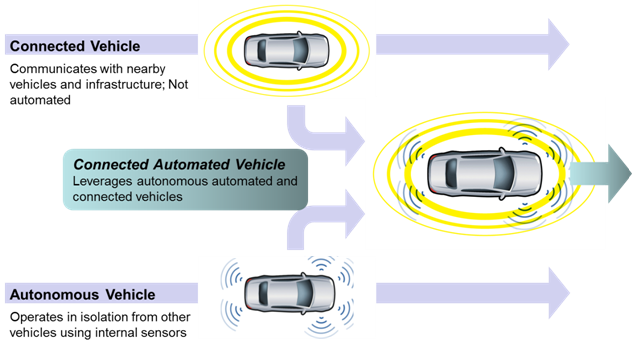
\includegraphics[width=13cm]{IV.png}}
\caption{网联车与自动驾驶车}
\label{fig:IV}
\end{figure}

将车路协同技术和无人驾驶技术融合,是智能车发展的必然趋势。新一代智能车不仅可以通过感知技术提高对驾驶环境的认知能力,还将通过网联技术实现信息交互,提升车辆运行效率、降低车辆能耗提升交通系统性等方面有极大的潜力。基于这样的平台,对于智能车的决策方案有望从单决策传统智能车决策方法,走向对多智车以群体行为效果为主的决策方案的研究,从而进一步提高系统整体的运行效率和安全性。

对于这样复杂系统的研究和群决策机理的分析,可以从相对简单的场景开始,再进一步向复杂场景进行推广。因此,本课题将以完全可控的无人车为研究对象,基于车路协同平台,研究多智能车系统在车辆交汇口的群决策问题。本课题的研究意义在于:

\begin{enumerate}[label=(\arabic*),wide=\parindent]
% \begin{enumerate}[label=(\arabic*),itemindent=\dimexpr\labelwidth+\labelsep\relax,leftmargin=0pt]
% \begin{enumerate}
\item 智能车是富有前景的未来交通工具,本课题将对智能车的应用奠定理论基础;
\item 车路协同平台为多智能车的群决策提供了支持,而群决策相比于个体决策能达到更高的通行效率,有必要对其理论进行研究;
\item 智能车于非智能车的混合驾驶将会是未来交通发展的必经阶段,本课题研究的多智能车场景是混合驾驶场景的基础;
\item 智能交通研究中的各种场景都可以作为多智能车群决策问题的背景,本课题所研究的交汇口场景是复杂场景研究的基础。
\end{enumerate}

\section{研究现状}
本章对于同本课题相关的研究进行文献综述。具体地,\ref{sec:VIC}节总结了世界范围内车路协同基础设施的最新进展,为多智能车的群决策提供支持;\ref{sec:self}节总结了无人车的发展历史和基本概念;\ref{sec:single}节对单智能车的运动学模型和决策问题进行了概述;\ref{sec:multi}对多智能车的决策问题进行了概述。

% 15 pages

% TODO: Is this necessary?

% \subsection{交通流理论}
%     交通流是研究
%     \subsubsection{交通流的分类}
%     交通流
%     Traffic flow can be divided into two primary types. Understanding what type of flow is occurring in a given situation will help you decide which analysis methods and descriptions are the most relevant.

%     The first type is called uninterrupted flow, and is flow regulated by vehicle-vehicle interactions and interactions between vehicles and the roadway. For example, vehicles traveling on an interstate highway are participating in uninterrupted flow.

%     The second type of traffic flow is called interrupted flow. Interrupted flow is flow regulated by an external means, such as a traffic signal. Under interrupted flow conditions, vehicle-vehicle interactions and vehicle-roadway interactions play a secondary role in defining the traffic flow.

%     \subsubsection{交通流描述参数}

%     \subsubsection{}
\subsection{车路协同系统的发展}
\label{sec:VIC}
车路协同通过部署新型基础设施,实现车车交互、车路交互,以提高交通系统的安全性和运行效率。近几年来,无人车技术,通信技术,GPS定位技术,以及云计算等新技术的发展在智能交通领域的应用,进一步推动了车路协同技术的应用与升级。

\begin{enumerate}[wide=\parindent]
\item \textbf{国外车路协同研究现状}

\textbf{美国  IntelliDrive} 美国车路协同系统(vehicle infrastructure integration, VII),后更名为 IntelliDrive,是由美国联邦公路局 (FHWA)、AASHTO、各州交通部 (State DOT)、汽车产业联盟、ITS American 等机构联合参与,着眼于安全性、交通机动性和环境友好性。项目在未来还将整合主动安全、电子支付等先进技术,进一步提高道路通行的效率和安全性。

\textbf{日本  SmartWay} 日本的车路协同系统 Smartway \cite{Hiroshi2005Smartway} 由23家企业与政府共同发起,其发展重点在整合日本各项 ITS的功能,促进基础道路设施改善、提高交通运输效率、并促进智能车(advanced safety vehicle, ASV)\cite{Chapman2010USING}的研发。该项目已经在东京区、三大都会区进行了试验,同时还能提供辅助驾驶、图像采集、停车场电子付费等服务。

\textbf{欧洲  eSafty} 该计划2003年9月得到欧盟委员会的认可并列入欧盟计划,旨在利用最新信息与通信技术,
加快研发并集成安全系统,为道路交通提供全面安全解决方案。欧洲自2010年,对智能车展开了实地测试。

\item \textbf{国内车路协同系统研究现状}

我国在车路协同方面的研究起步较晚。近年来,高校与科研单位逐步开展了车路协同技术的研究\cite{Tian2010A,Danno2009VEHICLE}。2010 年,国家“十二五” 高技术研究发展研究计划所支持的“智能车路协同关键技术研究”主题项目,是我国第一个国家级的车路协同项目。该项目由清华大学牵头,研究团队囊括了国内顶尖的科研院所和汽车制造企业,实力强劲。项目中,研究团队针对车车交互、车路交互、协同控制与大规模仿真等关键技术开展研究工作,获得了丰硕成果。在清华河北研究院廊坊实验场,建设了一条包含两个十字路口和一条1.3km实验路段的测试环境,用于车路协同应用和交互试验,取得了一系列成果。项目组还提出了基于车路协同技术我国新一代ITS 体系框架,突出了车路协同系统的核心地位,使得所有ITS 服务子系统均依托于车路协同系统的平台建立,形成一个高效的有机整体。
\end{enumerate}

\subsection{无人车}
\label{sec:self}

本节总结了无人车控制技术发展的历史,和无人车的自动程度分级,为后文具体综述无人车决策控制算法提供了背景知识。

\begin{enumerate}[wide=\parindent]
\item \textbf{无人车发展历程}

无人车技术具有悠久的历史。早在20世纪20年代,无人车的构想就已经出现\cite{Adrienne2016Your}。从20世纪80年代开始,关于无人车控制的理论研究陆续开始\cite{Dickmanns1988Dynamic}。1994年,作为 PROMETHEUS 工程\cite{eureka2016}的一部分,一辆名为 VaMP的无人车\cite{vamp2017}行驶了$1600$公里,其中$95\%$的路程是自动驾驶完成的。到2004年,为推动无人车技术的发展,第一次 DARPA 挑战在美国举办。挑战要求无人车自主完成长达150英里的越野赛道,与之前的无人车展示不同的是,比赛期间是不允许人工干预的。在此之后,又有许多关于无人车的比赛产生,值得一提的是在我国举办的 Intelligent Vehicle Future Challenges (IVFC)\cite{Xin2014China}。

\item \textbf{无人车自动程度等级}

SAE J3016 标准\cite{SO2014Taxonomy}将车辆自动化程度分为五个等级:

\textbf{等级0} 车辆完全由人控制;

\textbf{等级1} 包含基本驾驶辅助系统的车辆,例如自适应巡航控制系统,防抱死系统,电子稳定性控制\cite{Rajamani2011Vehicle}等;

\textbf{等级2} 包含高级辅助系统的车辆,例如危害最小化纵/横向控制系统\cite{Gerdes2001A},紧急制动系统\cite{Brannstrom2010Model,Vahidi2003Research}等;

\textbf{等级3} 车辆带有环境感知系统,能够在特定环境下全自动行驶,但在环境超出驾驶系统决策范围时仍需要人工干预,驾驶系统会让驾驶员接管并留出足够宽裕的转换时间;

\textbf{等级4} 车辆能够在特定环境中全自动行驶,并且当驾驶员没有响应接管请求时,仍能安全控制车辆;

\textbf{等级5} 在所有环境中都能够自动驾驶,不需要人为干预。

\end{enumerate}

\subsection{单智能车决策问题}
\label{sec:single}
本节讨论关于智能车决策控制的具体算法,主要讨论单个智能车的决策控制方法。其中\ref{sec:hierarchy}节给出了无人车决策问题的分层,\ref{sec:behavior}和\ref{sec:trajectory}节分别讨论了与本课题相关的行为决策和轨迹规划相关算法。

\begin{enumerate}[wide=\parindent]
\item \textbf{无人车决策层次}
\label{sec:hierarchy}

无人车的控制系统,本质上是一个自动决策系统,该系统能够从传感器获取信息流,并结合对道路拓扑、交通规则、车辆运动学、传感器模型的先验知识,决定能够控制汽车运动的输出量。研究者普遍将无人车的决策问题分解为不同的层次,解决每个层面的控制问题。该问题可以分解为以下四层:路径规划层、行为决策层、动作决策层和车辆控制层\cite{paden2016survey},如图\ref{fig:decision0}。

\begin{figure}[htbp]
\centering
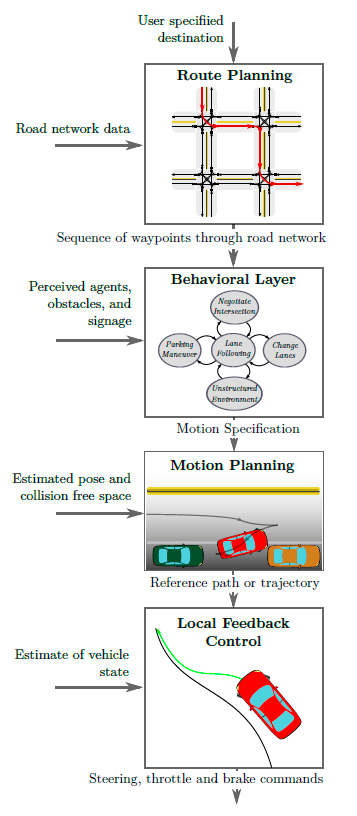
\includegraphics[width=9cm]{decision.png}
\caption{无人车决策层次\cite{paden2016survey}}
\label{fig:decision0}
\end{figure}

\textbf{路径规划层 } 这是无人车决策的最上层问题。通过将道路表示为有向网络,路径规划问题本质上就变成了一个最小费用流问题,可以采用 Dijkstra算法\cite{Dijkstra1959A},$A^*$启发式搜索\cite{Nilsson1969A}等。在路径规划的研究领域,目前已经出现了一系列算法,能够在经过一次预处理过后,在大陆规模的路网中以微秒量级输出最佳路径\cite{Goldberg2003Computing,Geisberger2012Exact}。

\textbf{行为决策层 } 当路径规划层求得了最佳路径之后,无人车需要根据路径进行导航,并和其他道路对象(人、车、障碍物等)进行交互。具体来说,输入一系列的路段,行为决策层需要根据感知到的路况信息(其他对象位置、信号灯等)决定驾驶行为(左转、右转、加速、减速、停车等)。由于周围环境和驾驶行为都可以被建模为有限集,可以使用有限状态机建模行为决策问题。其中状态为驾驶行为,状态转移由观察到的环境信息决定。

转移规则的学习可以使用传统的基于规则或基于统计的学习方法。在前述的 DARPA挑战赛中,大多数队伍都使用了基于规则的学习方法\cite{Buehler2009The}。近年来,由于人工智能的发展,业界也纷纷开始尝试使用深度学习、增强学习的方法,例如英伟达公司使用增强学习进行端到端无人车控制的工作\cite{Bojarski2016End}。

\textbf{轨迹规划层 } 当驾驶行为被确定后,选定的驾驶行为需要由轨迹规划层转化为特定的轨迹,提供给底层反馈控制单元沿轨迹运行。对于该路径可能存在障碍、曲率等一系列约束,优化的目标函数可能包括路径长度、人的舒适程度等。轨迹规划问题的精确解一般难以得到,在实际使用中往往进行数值近似。常用的轨迹规划方法有变分法、图搜索方法等。

\textbf{车辆控制层 } 确定轨迹之后,需要由反馈控制单元选择合适的致动输入来追踪轨迹。该领域研究集中在闭环系统的稳定性、鲁棒性和误差上,属于控制理论的研究范畴。

综合以上层次,无人车便可实现从路径到驾驶操作的控制。本课题研究的决策层面集中在行为决策和轨迹规划上,对路径规划和车辆反馈控制不做研究。其中\ref{sec:behavior}节总结了行为决策的相关算法,\ref{sec:trajectory}节总结了轨迹规划的相关算法。

\item \textbf{行为决策算法综述}
\label{sec:behavior}

\textbf{规则模型的建立 }
前文已经提到,由于车辆的行为可以定义为有限集合,行为决策可以使用有限状态机的方法。例如,Stanford大学在2007年 DARPA中参赛的无人车 Junior,建立了一个拥有13个状态的有限状态机进行车辆行为决策\cite{Montemerlo2008Junior}。其状态分别为:初始状态、前进、停止标志等待、路口等待、其他车辆等待、U形转弯、U形转弯等待、通过路口、停车导航、堵车、逃脱堵车、不匹配RNDF路网文件、任务完成。其各种状态的转移关系如图\ref{fig:junior}。在2007年 DARPA 比赛中胜出的 BOSS\cite{Baker2008Traffic}无人车采用了层次状态机的方法,其主要决策系统如图\ref{fig:boss}。BOSS的状态估计(State Estimator)和目标选择(Goal Selector)模块共同决定车辆运动的目标。其中状态估计模块输入车辆的地理位置和运行状态信息,用于估计车辆在路网中的相对位置。目标选择模块进一步根据设定的目标函数,选择车辆的当前道路行驶目标、下一个交叉口目标和未来计划目标,并交给车道行驶部分和交叉口处理部分进一步决策。根据不断生成的行动目标累积形成车辆动作。

\begin{figure}[htbp]
\centering
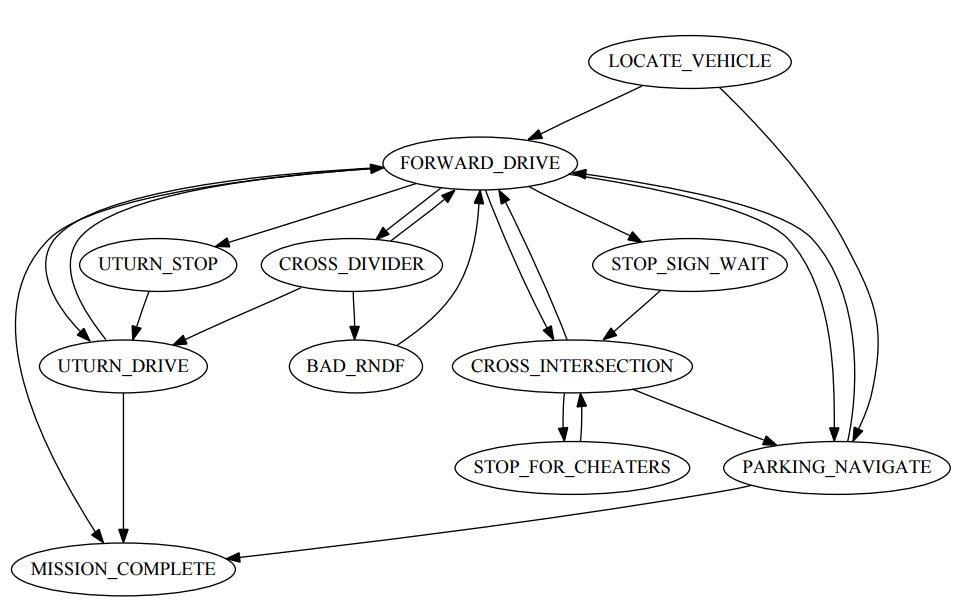
\includegraphics[width=10cm]{Junior.png}
\caption[Junior的状态转移图]{Junior的状态转移图\cite{Montemerlo2008Junior}}
\label{fig:junior}
\end{figure}

\begin{figure}[htbp]
\centering
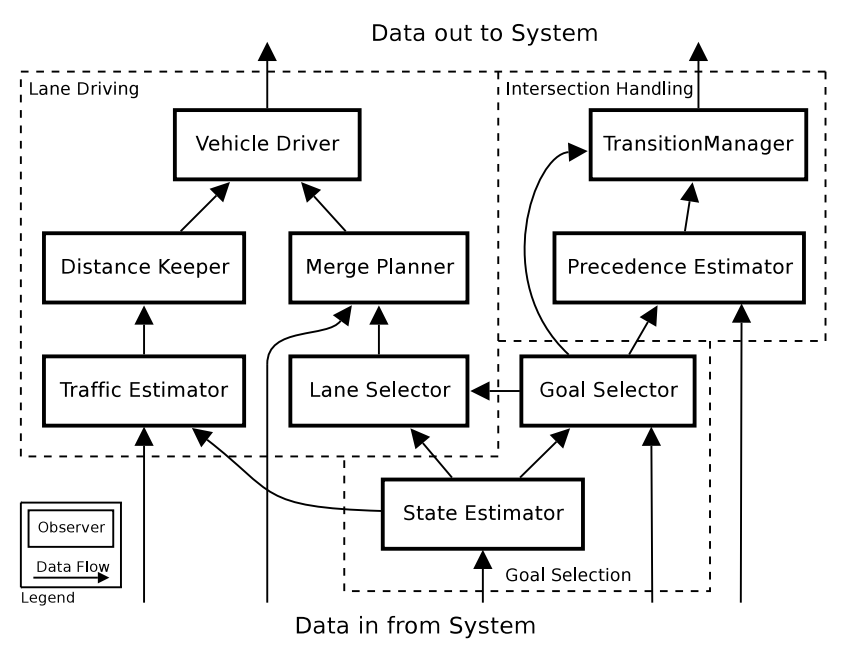
\includegraphics[width=10cm]{BOSS.png}
\caption[BOSS的行为决策流程]{BOSS的行为决策流程\cite{Baker2008Traffic}}
\label{fig:boss}
\end{figure}

这种状态机方法往往仅能在特定情况下正常工作,而现实中的交通场景变化多端,只依靠预先确定的状态和规则不能保证控制的安全性。

\textbf{规则学习方法 }
如果无人车可以很好的模拟人的驾驶行为,可以直接解决行为决策的问题。因此,行为决策和驾驶行为预测是紧密相关的,行为决策的规则可以从实际驾驶行为数据中进行学习。使用贝叶斯算法可以完成这一点。例如,Kumar P.等人\cite{Kumar2013Learning}使用贝叶斯方法对驾驶员数据进行分析,预测车道汇合时的驾驶员意图。Lidstrom K. 等人\cite{Lidstrom2008Model}指出动态贝叶斯网络(Dynamic Bayesian Model, DBN)可以用来处理不确定的时空依赖性。决策树也可以用于规则的学习。例如Schubert R.\cite{Schubert2012Evaluating}利用决策树能融知 识表示与获取于一身的优点,将决策树用不同驾驶行为机制的研究,以实现 对驾驶员行为的模拟再现。人工神经网络具有高度非线性映射能力,在智能控制中有广泛应用。例如 Chong L.等人\cite{Chong2013A}提出了一种基于模糊规则的神经网络从车辆轨迹预测驾驶员的驾驶行为。

诸如此类的规则学习方法还有很多种。这类方法在经过线下学习之后可以在各种场景下快速决定驾驶行为,但由于实际驾驶环境还有很多不确定性,对环境的感知也可能存在不一致的情况,对行为的决策最好能够考虑这种不确定性。

\textbf{不确定性的建模 }
考虑到其他车辆的行为是不确定的,行为决策系统经常使用概率模型,例如马尔科夫决策过程(Markov Decision Process, MDP)及其推广形式。\cite{Brechtel2011Probabilistic}即使用了MDP模型解决无人车的行为决策问题。另外一些工作将未观察到的驾驶场景和行人意图使用 partially-observable MDP (POMDB)建模,由此估计驾驶场景并进行行为决策。例如\citen{Ulbrich2013Probabilistic}提出了如图\ref{fig:POMDB}所示的两步决策过程,减小了传感器噪声对车道变换中行为决策的影响。

\begin{figure}[htbp]
\centering
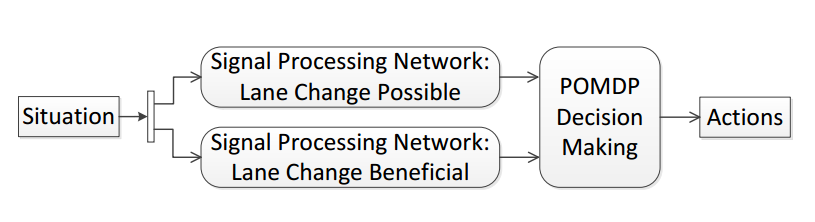
\includegraphics[width=13cm]{POMDB.png}
\caption[POMDB在车道转换中的决策过程]{POMDB在车道转换中的决策过程\cite{Ulbrich2013Probabilistic}}
\label{fig:POMDB}
\end{figure}

\item \textbf{轨迹规划算法综述}
\label{sec:trajectory}

轨迹规划问题又可以根据是否将时间当做自变量,分为路线(Path)规划和轨线(Trajectory)规划。其中路线规划获得的路线可表达为函数 $\sigma(\alpha): [0,1]\rightarrow \mathcal{X}$,其中$\mathcal{X}$为车辆的构形空间(Configuration Space,指规划范围内空间位置的集合)。对于轨线规划问题,获得的轨线可表达为函数 $\pi(t): [0, T]\rightarrow \mathcal{X}$,其中$T$为规划时限。

\textbf{路线规划 } 路线规划问题就是从初始构形开始,求得能够到达目标区域的满足全局和局部约束的路线。根据路线规划的目标,路线规划又可分为\textbf{可行路线规划}和\textbf{最优路线规划}。令$\mathcal{X}$表示车辆的构形空间,$\Sigma(\mathcal{X})$表示所有$[0,1]\rightarrow \mathcal{X}$的连续函数的集合,$\mathbf{x}_{\mathrm{init}}\in \mathcal{X}$表示初始构形,$X_{\mathrm{goal}}\subseteq \mathcal{X}$表示目标区域。车辆可达区域构成自由构形空间$\mathcal{X}_{\mathrm{free}}$。此外,车辆路线还需要满足一系列阶次的约束,表示为$D(\mathbf{x},\mathbf{x}',\mathbf{x}'', \dots)$,对于最优路线规划的描述如下:

\begin{definition}[最优路线规划]
\label{def:path}
给定五元组$(\mathcal{X}_{\mathrm{free}}, \mathbf{x}_{\mathrm{init}}, X_{\mathrm{goal}}, D, J)$ 找出$\sigma^*=$
\begin{equation}
\begin{aligned}
\underset{\sigma\in \Sigma(\mathcal{X})}{\arg\min}\quad & J(\sigma) & \\
\mathrm{subj. to} \quad & \sigma(0)=\mathbf{x}_{\mathrm{init}} \quad \mathrm{and} \quad \sigma(1)\in X_{goal} & \\
\quad & \sigma(\alpha)\in \mathcal{X}_{\mathrm{free}} & \quad \forall \alpha\in [0,1]\\
& D(\sigma(\alpha),\sigma'(\alpha),\sigma''(\alpha), \dots) & \forall \alpha\in [0,1]
\end{aligned}
\end{equation}
\end{definition}

最优路线规划已经被证明是 PSPACE难的问题\cite{Reif1979Complexity}。如果假设 $\mathrm{P}\neq \mathrm{NP}$,则不存在多项式复杂度的算法,能够在任何情况下解最优路线规划问题。对于求解可行路线规划,在1979年,Reif\cite{Reif1979Complexity}研究了完整车辆(holonomic vehicle,不存在非完整性约束)在二维、三维环境中寻找可行路线的问题,提出了一种多项式复杂度的算法。Canny\cite{Canny1988The}证明了用多边形表示自由构形空间,不存在高阶约束时,可行路线规划问题是PSPACE完全的。

对于最优路线规划,常见的目标是求得最短的无障碍路径。在该目标下,对于完整车辆,在二维多边形障碍的构形空间中存在多项式时间的算法\cite{Storer1994Shortest,Lozano1979An}。更准确地讲,存在复杂度为$O(n^2)$的算法,其中$n$为空间中车辆数目。该方法是基于可见性图的。

\textbf{轨线规划 } 与路线规划类似,最优轨线规划问题的定义如下:

\begin{definition}[最优轨线规划]
\label{def:trajectory}
给定六元组$(\mathcal{X}_{\mathrm{free}}, \mathbf{x}_{\mathrm{init}}, X_{\mathrm{goal}}, D, J, T)$ 找出$\pi^*=$
\begin{equation}
\begin{aligned}
\underset{\pi\in \Sigma(\mathcal{X})}{\arg\min}\quad & J(\pi) & \\
\mathrm{subj. to} \quad & \pi(0)=\mathbf{x}_{\mathrm{init}} \quad \mathrm{and} \quad \pi(1)\in X_{goal} & \\
\quad & \pi(t)\in \mathcal{X}_{\mathrm{free}} & \quad \forall t\in [0,1]\\
& D(\pi(t),\pi'(t),\pi''(t), \dots) & \forall t\in [0,1]
\end{aligned}
\end{equation}
\end{definition}

由于轨线规划是路线规划的推广,最优轨线规划仍是PSPACE难的。Canny和Reif\cite{Canny1987New}证明了对于有速度约束的完整车辆,在二维多边形障碍的共性空间中找到最短无障碍轨线是NP难的。注意到同样环境下的路线规划问题是存在$O(n^2)$算法的。该环境是无人车控制的典型环境。由于不存在有效的算法能够求得精确解,通常采用数值解法。

\textbf{轨迹规划的数值解法 }

常用的数值解法可以分为以下三大类:

\begin{enumerate}[label=(\arabic*),wide=\parindent]
% \begin{enumerate}
\item \textbf{变分法}(Variational methods)提取一组参数,将最优路线或轨线的求解问题转化为在该参数空间的搜索问题,优化的函数往往是非线性的。这种方法收敛较快,但不能保证收敛到全局最优。\citen{Ziegler2014Making}将优化问题转化为数值积分问题,并使用欧拉法优化。\citen{Darby2011An}进一步用一组基函数表示插值函数,获得了更快的收敛速度。对于变分法更详细的综述,参见\citen{Betts1998Survey}。

\item \textbf{图搜索算法}(Graph-search methods)将构形空间离散化为有限的顶点而生成图,图的边表示顶点之间的转移关系。最优路线或轨线的求解可转化为在图中求最小费用路径的问题。图\ref{fig:graph}为一个人工标定的车道图示例。生成该图除了人工标定,也可以从地理图片生成\cite{Backer2007Finding,Wang1996Approximation},或从观测到的构形空间采样生成\cite{Lavalle1999Rapidly,Glassman2010A}。获得了道路结构图之后,可以使用Dijkstra算法\cite{Dijkstra1959A}或$A^*$启发式搜索\cite{Hart2010A}。图搜索方法虽然能够获得全局最优,但得到的最优路径只是在由离散的构形空间点上的最优路径,而在整个构形空间上可能是次优的。有时这种方法甚至无法得到可行路径。

\item \textbf{递增搜索算法}(Incremental search methods)增量地寻找可行路径。如果存在可行路径,该方法在计算时间足够的情况下总能找到可行路径。若要求寻找最优路径,该方法可以进一步给出一列渐优的路径,逐渐收敛到最优路径。\citen{David1997Path}提出了一种基于可扩展空间树(expansive spaces tree, EST)的方法,每次随机从当前所有节点中选择一个扩展节点,在以该节点为中心的圆形区域采样得到扩展的节点。La Valle\cite{Lavalle1999Rapidly}提出了一种快速探索的随机扩展树(Rapid-exploring Random Tree, RRT),能够快速在高阶非完整系统中找到可行路径。

\end{enumerate}

\begin{figure}[htbp]
\centering
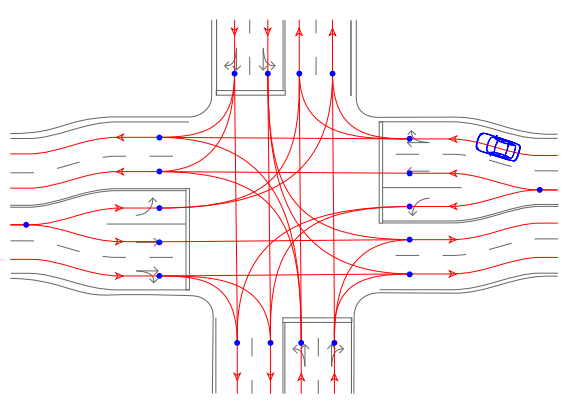
\includegraphics[width=8cm]{graph.png}
\caption{典型道路拓扑图}
\label{fig:graph}
\end{figure}
\end{enumerate}

\subsection{多智能车决策问题}
\label{sec:multi}
上述无人车研究均只涉及了单车的控制问题。如果在多车群决策系统中进行优化,即使使用简单的车辆模型,往往也能达到和单车分别决策相同,甚至更好的效果\cite{Cao2012An}。由于车路协同平台的发展,对于多智能车的协同控制,即群决策应用的需求也越来越大。多车的协同控制是具有广阔前景的研究领域。

多智能车协作问题是多智能体系统(Multi-Agent System, MAS)的具体应用。其控制方法可分为中心化方法和分布式方法两种。前者需要有强大的计算中心支持,一个中心需要处理大量车辆的决策问题。本质上,该方法是单车控制策略的拓展,仍可使用单车控制中的一系列方法进行类似的处理。而后者则将计算任务分配到每个车辆,省去了计算中心,但会使整个系统的结构和组织更为复杂。

由于本课题研究车道汇合处的决策问题,下面将针对车道汇合场景进行多智能车决策问题的综述。基于车路协同平台,车辆之间的通信方式、控制方式都和传统的单车决策、信号灯控制有很大不同。在该环境下,对车道汇合问题的研究主要分为三方面:

\begin{enumerate}[label=(\arabic*),wide=\parindent]
% \begin{enumerate}
\item 研究新的通信方式下如何提高交通通行效率和安全性;
\item 研究通信本身的可靠性和对车道汇合问题的影响;
\item 实验仿真车或其他机器人在汇合场景的表现。
\end{enumerate}

下文将对这三方面分别展开综述。

% \item \textbf{研究问题}
% 计划群决策的三个层次:
% 信息方面的决策
% 基于决策的决策
% 行为预测,决策协作?

\textbf{安全性和效率问题 }
根据前文单车轨迹规划的背景知识,车辆轨迹规划可以通过设计不同的目标函数而达到不同的优化效果。同样的,多车的轨迹规划问题也可以通过设计多车协作的整体目标来权衡安全性和效率。在较早的车道汇合研究中,\citen{Kanaris2001Strategies}将目标选取为优化交通流的分布,\citen{Raravi2007Merge}则着重优化车辆通过交叉路口的总时间,但忽略了车辆汇合的顺序问题,这可能造成不公平。\citen{Baselt2014Merging}则将公平性也作为一种目标,提出了一种名为\"自由流\"(free-flow)的公平性度量。为了考察多车协同的有效性,\citen{Xu2002Effects}研究了存在与不存在车间通信的情况下,汇合点上游车队长度的问题。\citen{Xu2003Simulation}考察了协同自主巡航系统(cooperative autonomous cruise control, C-ACC)和没有协同控制的自主巡航系统(autonomous cruise control, ACC)在汇合处对整体通行目标的影响。\citen{Wang2009Robust}总结了车辆在交汇口的标准问题、决策方法和通信算法。\cite{Gradinescu2007Adaptive}使用传统交通信号灯控制方案研究了存在车车通信时十字路口的控制问题。
\textbf{通信可靠性问题 }
\cite{Abbas2013Radio}讨论了车道汇合和交叉口场景中天线辐射模式对视野长度的影响。\citen{Uno1999A}提出了一种车道汇合处无人车的控制算法,并研究了通信时延对算法的影响。
\textbf{仿真实验 }
部分研究者从实验角度研究车辆在车道汇合场景的行为。如\citen{Sakaguchi1999Inter,Kolodko2003Cooperative}等工作很早(1999, 2003年)就开始研究存在车间通信的情况下,车辆在车道汇合、十字路口等场景的控制问题。而时间较近的一个实验\cite{Milanes2011Automated}也研究了类似的场景,展示了车车协同在路口汇合场景中的可行性。该实验是AUTOPIA\cite{Milan2011AUTOPIA}项目的一部分。

\subsection{总结}
从以上文献综述以及智能交通领域,尤其是多智能车协同控制领域近年的发展来看,可以得出以下结论:

\begin{enumerate}[label=(\arabic*),wide=\parindent]
% \begin{enumerate}
\item 行为决策问题还未解决。对于无人车控制的四个层次,整体路线规划已经有相当快速的算法,在轨迹追踪和反馈控制领域也有较为成熟的技术,但无人车行为决策的界限还很模糊,算法还不能适应各种场景。而这也是智能交通当今研究的重点领域之一。
\item 多智能车决策与实际联系较少。虽然多智能车的算法研究很早就开始了,并且在机器人编队领域有许多方法可以借鉴,但由于车辆的控制与基础设施密切相关,在没有统一通信标准时,许多场景只能靠假设,或进行纯理论的研究。仿真实验虽然在上世纪就已经开始,但实际道路中车辆通信的基础设施还不够完善,以至于十几年时间里,仿真内容仍然十分类似。当今车美国、欧洲纷纷提出了一些车路协同、多车协作的通信标准\cite{Chen2014Cooperative}。在这样的背景下,多车的决策控制问题又迎来了新的机遇与挑战。
\item 混合通行系统的协同控制问题研究很少。由于无人车技术的进步,未来很长一段时间的实际交通环境将由无人车和有人驾驶车辆共同参与。之前的研究要么着眼于驾驶员行为预测,要么研究多个完全可控车辆的车队等问题,在混合通行环境中的协同控制,或者混合通行环境对于智能车协同控制的影响还没有研究。
\end{enumerate}

\section{研究内容}
基于以上的研究现状调研,并结合自动化系实际,本课题拟采用自动控制理论中所学的最优控制方法对车道交汇路口进行建模和分析,使用变分法对模型进行求解,对于无法获得解析解的情况,使用数值分析和运筹学中所学的方法求得数值解。具体来说,研究内容有以下几点:
\begin{enumerate}[label=(\arabic*),wide=\parindent]
% \begin{enumerate}
\item 对于车道交汇口场景的建模,最重要的问题是如何选取目标函数。本课题尝试最小化通行时间和系统总能量的方法,并尝试了优先时间下界的优化和将时间、能量因素融合的方法;
\item 交汇口的车辆通行顺序是影响控制目标的一个重要因素。本课题将分析多种通行顺序决策方式。除了传统的先进先出策略,本课题将提出一种基于最优通行时间的排序方法,并与先进先出的方案进行比较分析;
\item 为了对课题中提出的算法进行仿真,而避免专业仿真软件的一些冗余设定,本文作者基于{\ttfamily Python}语言自主开发了一套仿真程序框架和一个简单的网页应用。
\end{enumerate}

\section{论文组织}
后文的组织结构如下:第\ref{cha:algorithm}章建立了车道汇合群决策系统的模型和约束条件,提出了目标函数,并运用安全性约束确定了通行时间的下限;第\ref{cha:solve}章运用变分法,在不同的约束条件下对模型进行求解,并描述了基于最优通行时间的排序原理;第\ref{cha:sim}在多种情况下对算法进行了仿真;第\ref{cha:sum}对本文进行了总结,并提出了未来的研究方向。
% !TEX root = ../main.tex
\chapter{车道汇合模型与群决策算法框架}
\label{cha:algorithm}
\section{车道汇合问题模型构建}
道路交汇口广泛存在于城市道路、高速公路中,是一种十分常见的交通场景。交汇的两条道路通常分为主路和辅路。其中主路通常有多条车道,路面较宽敞,车速快;辅路通常只有一条车道,车速较慢。按照我国现行交通法规,辅路车辆应在不影响主路车辆正常通行的情况下汇入主路。在主路车流密集,车速较高时,往往会造成辅路车辆停车等待的情况,带来了道路资源、燃油的浪费。若通过交汇口的车辆均由 CAV 构成,则有可能通过群体性的决策使交汇过程无需停车,同时减小通行时间和燃油损耗。

考虑如图\ref{fig:merge}所示的交汇路口。为了简化问题,考虑主路只有一条车道的情况。可能发生横向碰撞的区域成为交汇区,长度为$S$
。在控制区内,车辆之间、车辆与中央控制器之间允许交换信息并运行控制算法, 控制区起点
到交汇区起点的长度为$L$。
\begin{figure}[htbp]
\centering
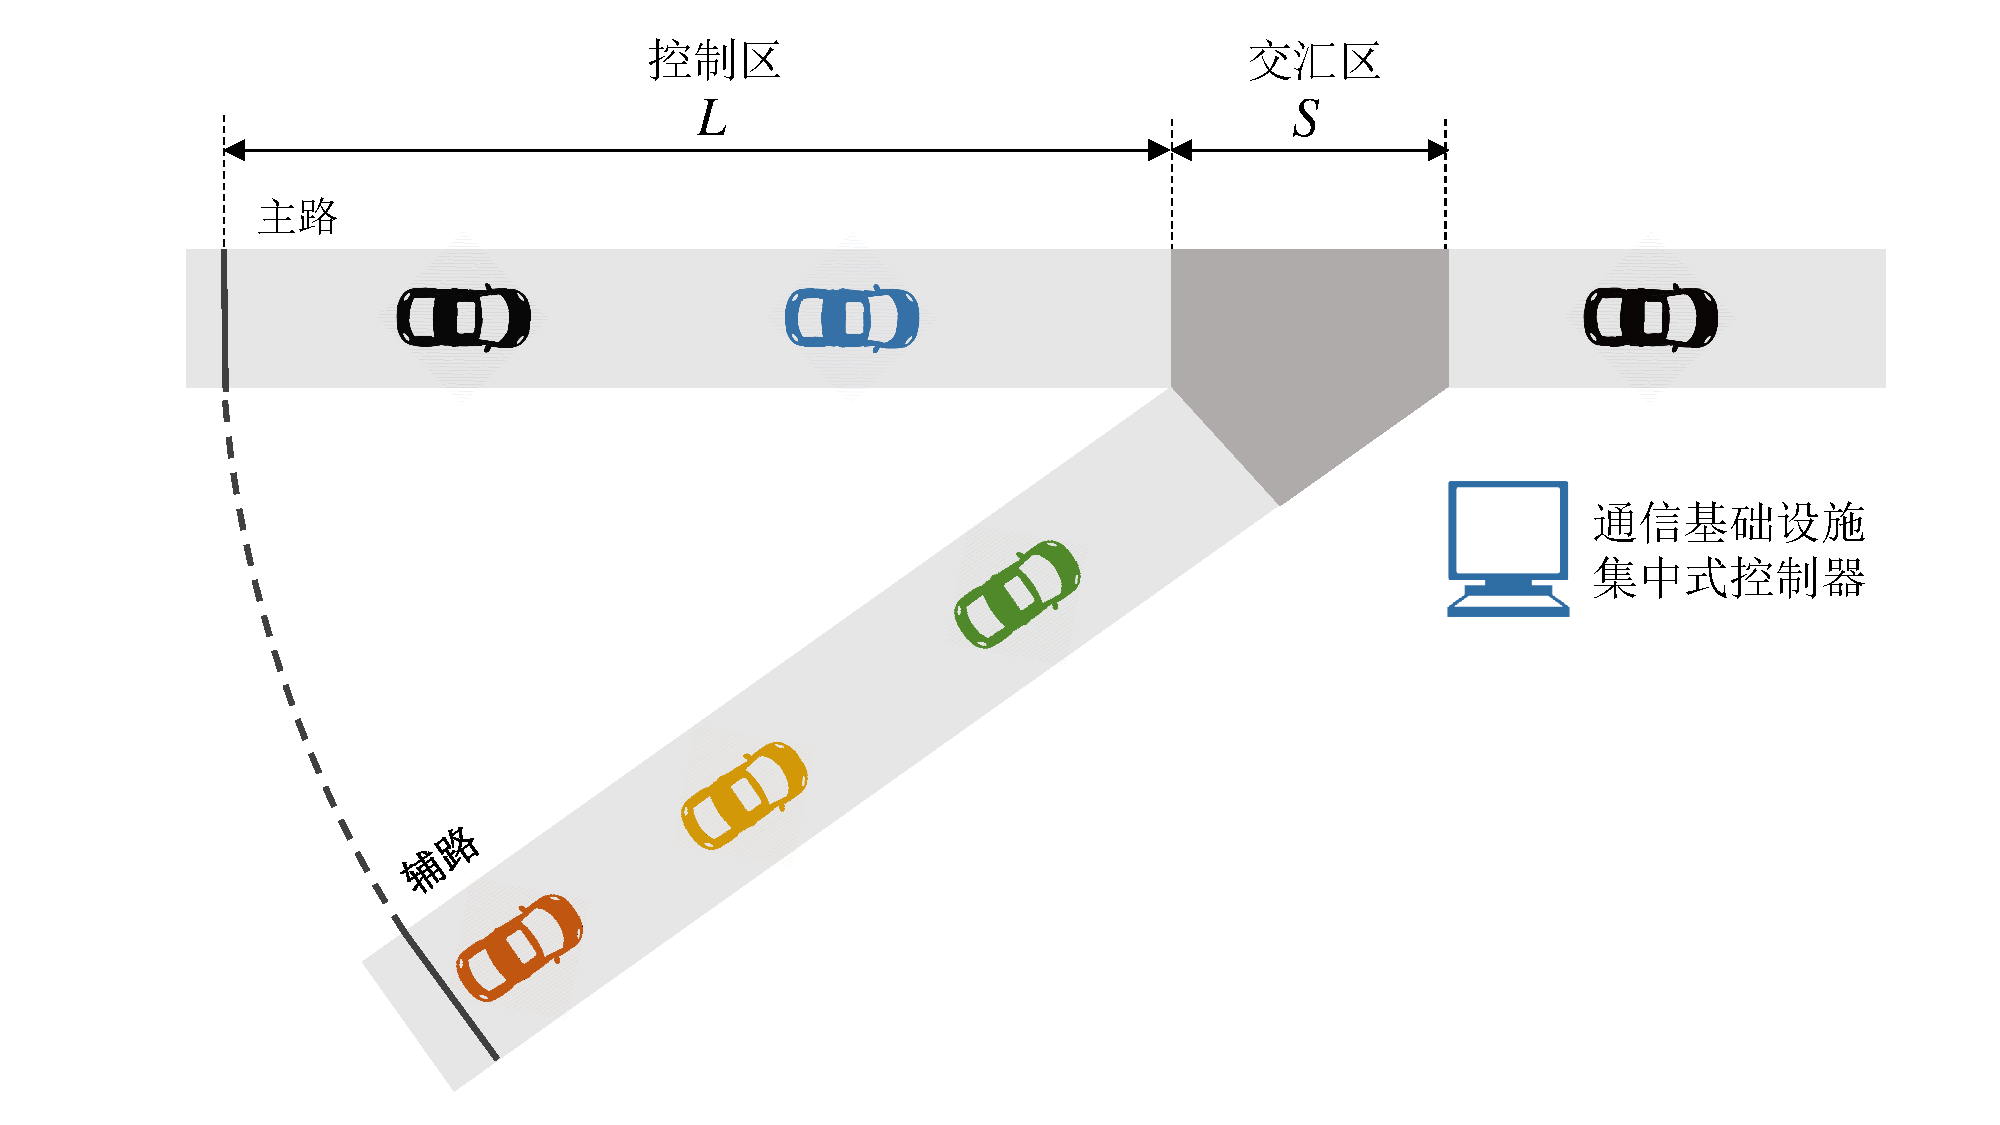
\includegraphics[width=14cm]{../figures/merge.pdf}
\caption{交汇路口示意图}
\label{fig:merge}
\end{figure}

\subsection{车辆状态方程}
假设在时刻 $t$时,位于控制区内的车辆具有某种编号 $\mathcal{N}(t)={1,\dots,N(t)}$,其中 $N(t)$为 $t$时刻控制区内车辆总数。对于每辆车$i\in \mathcal{N}(t)$,系统状态方程为
\begin{equation}
\dot{x}_i=f(t,x_i,u_i),\quad x_i(t_i^0)=x_i^0,
\end{equation}
其中$x_i(t)$,$u_i(t)$分别为第$i$辆车在$t$时刻的状态量和控制量。对于本课题讨论的无人车控制,假定车辆的轨迹已经确定,无需控制方向,只需控制速度。为了保证速度的连续性,选取控制量为加速度,则控制量与状态量的关系为,
\begin{equation}
\begin{gathered}
\dot{p}_i=v_i(t)\\
\dot{v}_i=u_i(t)
\end{gathered}
\label{eq:state}
\end{equation}
其中 $p_i(t)\in \mathcal{P}_i$,$v_i(t)\in \mathcal{V}_i$,$u_i(t)\in \mathcal{U}_i$分别为第 $i$辆车在 $t$时刻的位置,速度和加速度。由于轨迹事先已确定,只需要两个标量 $p_i$与 $v_i$即可确定当前车辆的位置和速度。二者构成了车辆的状态向量 $x_i(t)=[p_i(t), v_i(t)]^\mathrm{T}\in \mathcal{X}_i$,$\mathcal{X}_i=\mathcal{P}\times\mathcal{V}$,并定义进入控制区的初始状态为$x_i^0 = [0, v_i^0]^\mathrm{T}$。

对于实际运行的车辆,其速度和加速度均有限,表达为以下约束,
\begin{equation}
\begin{aligned}
u_{i,\min}\leq u_i(t)\leq u_{i,\max}&, \quad \text{and}\\
0\leq v_{\min}\leq v_i(t)\leq v_{\max}&, \quad \forall t\in[t_i^0, t_i^\mathrm{f}]
\end{aligned}
\label{eq:single_constraint}
\end{equation}
其中 $t_i^\mathrm{f}$为第 $i$辆车离开交汇区的时刻,即控制算法结束的时刻。 $u_{i,\min}$,$u_{i,\max}$分别为第$i$辆车的最小、最大加速度,$v_{\min}$,$v_{\max}$为道路的最低、最高限速。为简单起见,考虑同质车辆,所有CAV均具有相同的最小、最大加速度,即$u_{i,\min}=u_{\min}$,$u_{i,\max}=u_{\max}$。

\subsection{安全性约束与假设}
上一节建立了每辆车的状态方程和单车的约束条件,本节考虑车辆之间的约束关系。

控制算法首先要保证车辆之间不发生追尾。对同一车道上的车辆,定义安全距离$\delta < S$,同车道车辆之间不追尾的约束可以表示为,
\begin{equation}
s_i(t)=p_k(t)-p_i(t)\geq \delta, \ \forall t\in [t_i^0, t_i^\mathrm{f}],
\label{eq:colli_rear}
\end{equation}
其中$k$表示与$i$在同一车道的前一辆车的编号。上式涵盖了控制区、交汇区不发生同车道追尾的约束条件。

车辆仅在交汇区可能与对路车辆发生横向碰撞。给出如下定义:
\begin{definition}
对所有$i\in \mathcal{N}(t)$,定义第 $i$辆车的{\heiti 可能碰撞集} $\Gamma_i$为可能发生横向碰撞的$i$车位置构成的集合,即
\begin{equation}
\Gamma_i\triangleq \{p_i(t)\in[L,L+S],\  \forall t\in [t_i^\mathrm{m},t_i^\mathrm{f}]\}.
\end{equation}
其中$t_i^\mathrm{m}$为第$i$辆车离开控制区,进入交汇区的时刻。
\end{definition}
为了避免横向碰撞,对任意不在同一条路上的两辆车 $\forall i,j\in \mathcal{N}(t)$,给出如下约束:
\begin{equation}
\Gamma_i\cap \Gamma_j=\varnothing, \ \forall t\in [t_i^\mathrm{m},t_i^\mathrm{f}].
\label{eq:colli_lateral}
\end{equation}
上式要求来自相互交汇的两条路上的车辆不能同时出现在交汇区。这个约束必能保证车辆在交汇区不发生横向碰撞,但当交汇区的长度很长时,约束可能过强,没有必要。在下面的章节中将讨论如何放松该约束。

在定义优化目标之前,对控制算法做以下假设。
\begin{assumption}
进入控制区的车$i$满足约束式\ref{eq:single_constraint},\ref{eq:colli_rear}。
\label{ass:restrict}
\end{assumption}
\begin{assumption}
CAV在交汇区保持匀速行驶,且速度相同,即$v_i(t) = v_i(t_i^\mathrm{m}) = v_i(t_i^\mathrm{f}) = v_\mathrm{d}, \ \forall t\in [t_i^\mathrm{m},t_i^\mathrm{f}]$,其中$v_\mathrm{d}$为期望速度。由此可得
\begin{equation}
t_i^\mathrm{f}=t_i^\mathrm{m} + \frac{S}{v_\mathrm{d}}.
\end{equation}
\label{ass:smooth}
\end{assumption}
\begin{assumption}
忽略CAV之间信息传输的延时和错误。
\label{ass:time}
\end{assumption}

在以上假设中,假设\ref{ass:restrict}保证了初始状态的可行性。假设\ref{ass:smooth}忽略了交汇区的速度变化,且假设车辆在进入交汇区之前已经调整到了期望速度$v_\mathrm{d}$。该速度可以根据路段的限速事先给定。这是为了方便讨论交汇区的不碰撞约束,实际情况与此有一定差别。后文将对此展开进一步讨论。假设\ref{ass:time}保证车辆之间信息交互是实时且准确的。但本文的模型在信息的延时和错误处于有限范围内,仍可进行扩展。

\section{群决策算法框架}
% 这里加一段优化目标的综述
\subsection{时间序列的确定}
在假设\ref{ass:smooth}下,考虑到约束式\ref{eq:colli_rear}与式\ref{eq:colli_lateral},可以由$t_{i-1}^\mathrm{m}$确定$t_i^\mathrm{m}$的下界。考虑以下几种情况:
\paragraph{情况一} $i$车与 $i-1$车在同一车道,此时前后车只需保持安全距离,当$i-1$车驶过$\delta$距离后,$i$车便可进入交汇区。由此可得,
\begin{equation}
t_i^\mathrm{m}=t_{i-1}^\mathrm{m} + \frac{\delta}{v_\mathrm{d}}
\label{eq:t_case1}
\end{equation}
\paragraph{情况二}  $i$车与 $i-1$车在不同车道,由式\ref{eq:colli_lateral},当$i-1$车完全驶过交汇区后,$i$车才能进入交汇区。由此可得,
\begin{equation}
t_i^\mathrm{m}=t_{i-1}^\mathrm{m} + \frac{S}{v_\mathrm{d}}
\label{eq:t_case2}
\end{equation}

上述情况二满足了式\ref{eq:colli_lateral}所要求的不同车道不同时出现在交汇区的要求。若交汇区比较长,该要求可以适当放松为,使不同车道间车辆交汇后相距为 $r < S$,$r$为不同车道保证不发生横向碰撞的安全距离。在实际道路条件下,安全距离应随着速度的增加而适当增大。由于交汇区车速仍可视为保持期望速度 $v_\mathrm{d}$,$r$也可以作为常数而预先确定下来。情况二对应的时间关系变为,
\begin{equation}
t_i^\mathrm{m}=t_{i-1}^\mathrm{m} + \frac{r}{v_\mathrm{d}}
\label{eq:t_case2r}
\end{equation}

另外,对于不存在前车的第一辆车,其到达交汇区时间 $t_1^\mathrm{m}$可由优化目标解出。这将在下文进一步讨论。

\subsection{优化目标建立}
研究CAV的决策问题,就是在控制量满足一定约束的情况下,对每辆车给出一列控制量输入$u_i(t)$对于车道汇合的场景,一般优化目标包含最小化控制量的输入和最小化平均通行时间。\cite{Rios2016Automated}将二者包含在同一目标函数中,表达为,
\begin{equation}
\begin{aligned}
&\min_{u_i\in \mathcal{R}_i}\left(w_1\frac12\sum^{N(t)}_{i=1}\int_{t_i^0}^{t_i^\mathrm{f}}C_i\left(u_i\left(t\right)\right)\mathrm{d}t + w_2\sum_{i=2}^{N(t)}|t_i^\mathrm{m}(u_{(1:i)}(t))-t_{i-1}^\mathrm{m}(u_{(1:i-1)}(t))|\right),\\
&
\begin{aligned}
\text{Subject to:} & \quad \mbox{\ref{eq:state}}, \quad \forall i\in \mathcal{N}(t),\\
& \quad \mbox{\ref{eq:colli_lateral}}, \quad \forall i,j \in \mathcal{N}(t), i\neq j.
\end{aligned}
\end{aligned}
\label{eq:two_item_obj}
\end{equation}
其中$w_1$,$w_2$为调整两项权重的比例系数,$t_i^\mathrm{m}(u_{(1:i)}(t))$表示$i$车的$t_i^\mathrm{m}$可能与之前所有车的控制量输入都有关。$\mathcal{R}_i$定义如下:
\begin{definition}
对每辆车$i$,定义该车的{\heiti 控制区间}$\mathcal{R}_i$为,
\begin{equation}
\begin{gathered}
\mathcal{R}_i\triangleq\{u_i(t)\in[u_{\min}, u_{\max}]\ |\ p_i(t)\leq p_k(t)-\delta, v_i(t)\in[v_{\min}, v_{\max}],\\
\forall i \in \mathcal{N}, |\mathcal{N}(t)|>1, \forall t \in [t_i^0, t_i^\mathrm{f}]\ \}.
\end{gathered}
\end{equation}
\label{def:possible_u}
\end{definition}
定义\ref{def:possible_u}给出了可能的控制量输入集合。

式\ref{eq:two_item_obj}的第一项表示由控制量输入造成的损失,$C_i(u_i(t))$为控制量输入$u_i(t)$的某种函数。第二项为前后车进入交汇区时间差之和,该值越小,交汇路口吞吐量就越大。对于本文的优化问题,假设所有车辆均按照式\ref{eq:t_case1},\ref{eq:t_case2}(或\ref{eq:t_case2r})确定的时间下限通行,则可以略去目标函数式\ref{eq:two_item_obj}中的时间相关项,保留控制量相关项。选取目标为最小化控制量输入的平方\cite{Malikopoulos2016A,Rios2016Automated},即
\begin{equation}
J(\mathbf{u})=\frac12\int_{t_i^0}^{t_i^\mathrm{m}}u_i^2\mathrm{d}t
\label{eq:one_item_obj}
\end{equation}
其中$\mathbf{u}$为所有车控制量输入函数构成的向量。
% !TEX root = ../main.tex
\chapter{车道汇合场景的单车最优控制}
\label{cha:solve}

在上一章中已经给出了模型的目标函数,并且提到需要对每辆车求解一个控制量输入$u_i(t)$,使得$J(\bm{u})$达到最小。注意到$u_t(t)$实际上是关于时间$t$的函数,$J(\bm{u})$实际上是函数的函数,数学上称为泛函。求泛函的极值需要用到变分法的相关知识。本章先对泛函与变分法进行简要说明,之后运用该方法求解不同情况下泛函的极值,得到决策控制方法。

\section{泛函与变分法}
泛函的概念最早在变分法中出现,并广泛应用于最优控制的相关问题中。

\subsection{泛函与泛函的变分}
抽象空间理论将泛函定义为向量空间上的实值函数,而在最优控制中往往限定为函数集上的实值函数。定义如下,
\begin{definition}[泛函]
函数集$\mathcal{U}(x)$,到实数集$\mathbb{R}$的映射$J: \mathcal{U}\rightarrow \mathbb{R}$称为函数集$\mathcal{U}$上的{\heiti 泛函},即,
\begin{equation}
J=J[u(x)], \ u(x)\in \mathcal{U}(x).
\end{equation}
\end{definition}
泛函的变分与函数的微分类似。首先需要定义函数的变分,定义如下,
\begin{definition}[函数的变分]
设$u(x), u_0(x) \in \mathcal{U}(x)$,{\heiti 函数的变分}定义为
\begin{equation}
\delta u(x)=u(x) - u_0(x)
\end{equation}
\end{definition}
由以上定义知,函数的变分仍是$x$的函数。另外根据泛函定义,函数集$\mathcal{U}(x)$应是向量空间,对加法和数乘封闭,因此$\delta u(x)\in \mathcal{U}(x)$。
之后定义泛函的连续性如下,
\begin{definition}[泛函的连续性]
$\forall \varepsilon > 0$,$\exists \delta > 0$,对于$\forall u(x), d(u,u_0)<\delta$有
\begin{equation}
\Delta J[u(x)]=J[u(x)+\delta u(x)]-J[u(x)] < \delta
\end{equation}
其中$d(u,u_0)$为函数空间$\mathcal{U}$上定义的某种范数,则称泛函$J[u(x)]$在范数$d$下,在$u_0(x)$连续。
\end{definition}
泛函的变分定义如下,
\begin{definition}[泛函的变分]
泛函的增量若能表示为
\begin{equation}
\Delta J[u(x)]=L[u(x),\delta u(x)] + \gamma[u(x), \delta u(x)],
\end{equation}
其中$L[u(x),\delta u(x)]$是$\delta u(x)$的线性连续泛函,$\gamma[u(x), \delta u(x)]$是$\delta u(x)$的高阶无穷小,则称$L[u(x),\delta u(x)]$为泛函$J[u(x)]$的变分,记为
\begin{equation}
\delta J = L[u(x),\delta u(x)]
\end{equation}
\end{definition}
关于线性连续泛函的概念,以及泛函变分更严谨的定义,参见泛函分析的教材\cite{PETERD2007Functional}。

\subsection{变分法}
求泛函极值的方法称为变分法。泛函极值的定义与函数极值类似。下面不加证明地给出如下定理:
\begin{theorem}
若泛函$J[u(x)]$在$u_0(x)$有极值,则
\begin{equation}
\delta J[u_0(x)]=0
\end{equation}
\end{theorem}
注意,上述定理只是泛函取极值的必要条件。至于是否存在极值,是极大还是极小值,需要根据实际问题的性质确定。

变分学中有如下三类基本问题。三者区别在于泛函形式不同,而目标都是求泛函极小值。
\paragraph{拉格朗日(Lagrange)问题} 泛函形式为
\begin{equation}
J = \int_{t_0}^{t_\mathrm{f}}F(t,x,\dot{x})\mathrm{d}t,
\end{equation}
其中$t_0$为初始时间,$t_f$为终端时间。
\paragraph{梅耶(Mayer)问题} 泛函形式为
\begin{equation}
J=\theta[x_\mathrm{f},t_\mathrm{f}].
\end{equation}
该泛函是终端时间$t_\mathrm{f}$和终端函数$x_\mathrm{f}=x(t_mathrm{f})$的函数。
\paragraph{波尔查(Bolza)问题} 泛函形式为
\begin{equation}
J=\theta[x_\mathrm{f},t_\mathrm{f}]+\int_{t_0}^{t_\mathrm{f}}F(t,x,\dot{x})\mathrm{d}t.
\end{equation}
可见,前两者是后者的特殊形式。

\subsection{最优控制的必要条件}
最优控制问题常写作如下形式的波尔查问题
\begin{equation}
J(\bm{u})=\theta[t_\mathrm{f},\bm{x}_\mathrm{f}]+\int_{t_0}^{t_\mathrm{f}}L[\bm{x}(t),\bm{u}(t),t]\mathrm{d}t,
\end{equation}
其状态方程和初始状态为
\begin{equation}
\dot{\bm{x}}=\bm{f}[\bm{x}(t),\bm{u}(t),t], \quad \bm{x}(t_0)=\bm{x}_0.
\end{equation}
定义{\heiti 哈密顿函数}为
\begin{equation}
H(\bm{x},\bm{u},\bm{\lambda},t)=L(\bm{x},\bm{u},t)+\bm{\lambda}^\mathrm{T}\bm{f}(\bm{x},\bm{u},t),
\end{equation}

下面针对上述波尔查问题的形式,给出几种情况下的最优控制必要条件。若最优控制的损失函数退化为拉格朗日或梅耶问题的形式,其必要条件也可以相应得出。
\\
\begin{enumerate}
\item {\heiti 终端自由,$t_\mathrm{f}$给定的情形}
\\ 最优控制的必要条件为
\begin{gather}
\frac{\partial H}{\partial\bm{u}}=0,\label{eq:nc:control}\\
\dot{\bm{\lambda}}=-\frac{\partial H}{\partial\bm{x}},\label{eq:nc:company}\\
\bm{\lambda}(t_\mathrm{f})=\left. \left[\frac{\partial \theta}{\partial \bm{x}}+\frac{\partial \bm{g}^\mathrm{T}}{\partial \bm{x}}\bm{\mu}\right]\right|_{t_\mathrm{f}},\label{eq:nc:final}\\
\dot{\bm{x}}=\bm{f}(\bm{x},\bm{u},t),\\
\bm{x}(t_0)=\bm{x}_0.\label{eq:nc:last}
\end{gather}
其中式\eqref{eq:nc:control}也被称作{\heiti 控制方程},式\eqref{eq:nc:company}也被称作{\heiti 伴随方程}。若退化为拉格朗日问题,则$\theta[t_\mathrm{f},\bm{x}_\mathrm{f}]\equiv 0$,式\eqref{eq:nc:company}变为
\begin{equation}
\bm{\lambda}(t_\mathrm{f})=0.
\end{equation}

\item {\heiti 终端受限,$t_\mathrm{f}$给定的情形}
\\设终端约束条件为
\begin{equation}
\bm{g}(\bm{x}_\mathrm{f},t_\mathrm{f})=0,
\end{equation}
最优控制的必要条件为
\begin{gather}
\frac{\partial H}{\partial\bm{u}}=0,\label{eq:cc:control}\\
\dot{\bm{\lambda}}=-\frac{\partial H}{\partial\bm{x}},\label{eq:cc:company}\\
\bm{\lambda}(t_\mathrm{f})=\left. [\frac{\partial \theta}{\partial \bm{x}}+\frac{\partial \bm{g}^\mathrm{T}}{\partial \bm{x}}\bm{\mu}]\right|_{t_\mathrm{f}},\label{eq:cc:final}\\
\dot{\bm{x}}=\bm{f}(\bm{x},\bm{u},t),\\
\bm{x}(t_0)=\bm{x}_0.\label{eq:cc:last}
\end{gather}
其中$\bm{\mu}$为一个待定乘子。对比式\eqref{eq:cc:final}与式\eqref{eq:nc:final}可知,终端受限情况下,终端条件会发生变化。

\item {\heiti 终端受限,$t_\mathrm{f}$自由的情形}
\\最优控制的必要条件为
\begin{gather}
\frac{\partial H}{\partial\bm{u}}=0,\label{eq:cn:control}\\
\dot{\bm{\lambda}}=-\frac{\partial H}{\partial\bm{x}},\label{eq:cn:company}\\
\bm{\lambda}(t_\mathrm{f})=\left. \left[\frac{\partial \theta}{\partial \bm{x}}+\frac{\partial \bm{g}^\mathrm{T}}{\partial \bm{x}}\bm{\mu}\right]\right|_{t_\mathrm{f}},\label{eq:cn:final}\\
\left. \left[H+\frac{\partial\theta}{\partial t}+\bm{\mu}^\mathrm{T}\frac{\partial\bm{g}}{\partial t}\right]\right|_{t_\mathrm{f}}=0,\label{eq:cn:final2}\\
\dot{\bm{x}}=\bm{f}(\bm{x},\bm{u},t),\\
\bm{x}(t_0)=\bm{x}_0.\label{eq:cn:last}
\end{gather}
与之前的情形相比,该情形多了一个终端条件以确定$t_\mathrm{f}$。
\end{enumerate}

\section{最优控制问题求解}
\label{sec:solve}
运用上述最优控制的必要条件,可求解本课题的车道汇合群决策模型,获得最优控制策略。下面三小节分别考虑三种情形,其中\ref{ssec:noc}节首先研究控制量和状态量无约束,且终端时间固定的简单情形;\ref{ssec:freetf}节研究控制量和状态量无约束,终端时间自由的情形;\ref{ssec:c}研究控制量和状态量存在约束的情形。

\subsection{无约束情形}
\label{ssec:noc}
本节中的无约束是指对每辆CAV均不限制最大加速度和速度。另外,终端时间事先给定。式\eqref{eq:one_item_obj}在这种情形下,设$t_i^{0}=0$并省略所有下标$i$,最优控制问题的形式为
\begin{gather}
\min_{u} J(u)=\int_{0}^{t^\mathrm{m}}L(p,v,u,t)\mathrm{d}t=\int_{0}^{t^\mathrm{m}}\frac12 u^2\mathrm{d}t,\label{eq:noc:first}\\
p(0)=0, v(0)=v_0,\label{eq:noc:start}\\
p(t^\mathrm{m})=L, v(t_\mathrm{m})=v_\mathrm{d},\label{eq:noc:end}\\
\dot{p}=v, \dot{v}=u. \label{eq:noc:last}
\end{gather}
其中式\eqref{eq:noc:first}为目标函数,式\eqref{eq:noc:start}为初始状态,式\eqref{eq:noc:end}为终端约束,式\eqref{eq:cc:last}为系统状态方程。该问题是终端受限,$t_\mathrm{f}$给定的最优控制问题,必要条件为式\eqref{eq:cc:control}---\eqref{eq:cc:last}。该问题的哈密尔顿函数为,
\begin{equation}
H(p,v,u,t)=\frac12 u^2+\lambda^\mathrm{p}v + \lambda^\mathrm{v}u.
\end{equation}
由伴随方程得
\begin{align}
\dot{\lambda}^\mathrm{p}&=-\frac{\partial H}{\partial p}=0, \label{eq:dlp}\\
\dot{\lambda}^\mathrm{v}&=-\frac{\partial H}{\partial v}=-\lambda^\mathrm{p}. \label{eq:dlv}
\end{align}
由控制方程可得
\begin{equation}
\frac{\partial H}{\partial u}=u+\lambda^\mathrm{v}=0,
\label{eq:uwrtlv}
\end{equation}

式\eqref{eq:dlp}说明$\lambda^\mathrm{p}$为常数,设$\lambda^\mathrm{p}=a$,则可设$\lambda^\mathrm{v}=-(at+b)$,再由式\eqref{eq:uwrtlv}可得
\begin{equation}
u^*(t)=at+b,
\label{eq:ut}
\end{equation}
即在该情形下,最优的控制策略是加速度为时间的线性函数。注意在终端受限,$t_\mathrm{f}$自由情形的必要条件中还有关于$\bm{\lambda}$末状态的方程,但该方程额外引入了待定参数$\bm{\mu}$,实际上对求解最优控制不起作用,因此无需列出。
在该控制策略下,速度和位移与时间的关系可分别表达为时间的二次、三次函数
\begin{gather}
v^*(t)=\frac12at^2+bt+c,\\
p^*(t)=\frac16at^3+\frac12bt^2+ct+d.
\end{gather}
以上$a,b,c,d$均为待定常数,可以根据初始条件式\eqref{eq:noc:start}和终端条件式\eqref{eq:noc:end}得出。可列写如下方程
\begin{equation}
\begin{bmatrix}
\frac16t^3 & \frac12t^2 & t & 1 \\
\frac12t^2 & t & 1 & 0 \\
\frac16(t^\mathrm{m})^3 & \frac12(t^\mathrm{m})^2 & t^\mathrm{m} & 1 \\
\frac12(t^\mathrm{m})^2 & t^\mathrm{m} & 1 & 0
\end{bmatrix}\cdot
\begin{bmatrix}
a\\b\\c\\d
\end{bmatrix}
 = \begin{bmatrix}
p(t)\\v(t)\\p(t^\mathrm{m})\\v(t^\mathrm{m})
\end{bmatrix}.
\label{eq:noc:array}
\end{equation}
令$t$为进入控制区的时刻,则可以由初末状态,根据以上方程解出参数。注意,以上方程对每辆CAV都可以单独列写,即每辆车单独计算自己的控制策略。

\subsection{终端时间自由情形}
\label{ssec:freetf}
在第\ref{ssec:time_series}节曾提到,对于头一辆车,终端时间是待定的,而后面的车辆可以在预先确定通过顺序的情况下,由前一辆车的通过时间按照式\eqref{eq:t_case1},式\eqref{eq:t_case2}(或式\eqref{eq:t_case2r})确定。头一辆车的优化问题是一个终端受限,$t_\mathrm{f}$自由的最优控制问题,必要条件为式\eqref{eq:cn:control} $\sim$ 式\eqref{eq:cn:last}。问题的表述如式\eqref{eq:noc:first} $\sim$ 式\eqref{eq:noc:last}。这里将末态约束写为向量函数式
\begin{equation}
\bm{g}(p(t^\mathrm{m}),v(t^\mathrm{m}),t^\mathrm{m})=
\begin{bmatrix}
p(t^\mathrm{m})-L\\
v(t^\mathrm{m})-v_\mathrm{d}
\end{bmatrix}.
\end{equation}
由伴随方程和控制方程仍可解出$u(t)$为线性形式,如式\eqref{eq:ut}。下面需要终端方程来确定$t^\mathrm{m}$。

由终端条件式\eqref{eq:cn:final}和式\eqref{eq:cn:final2},
\begin{align}
\lambda^\mathrm{p}(t^\mathrm{m})=\frac{\partial \bm{g}^\mathrm{T}}{\partial p}\bm{\mu}=\mu^\mathrm{p},\label{eq:freetf:f1}\\
\lambda^\mathrm{v}(t^\mathrm{m})=\frac{\partial \bm{g}^\mathrm{T}}{\partial v}\bm{\mu}=\mu^\mathrm{v},\label{eq:freetf:f2}\\
\left. H+\mu^\mathrm{p}v+\mu^\mathrm{v}u\right|_{t^\mathrm{m}}=0.\label{eq:freetf:f3}
\end{align}
将式\eqref{eq:freetf:f1},式\eqref{eq:freetf:f2}及$u=-\lambda^\mathrm{v}$代入式\eqref{eq:freetf:f3},整理得
\begin{equation}
-\frac32(\lambda^\mathrm{v}(t^\mathrm{m}))^2+2\lambda^\mathrm{p}(t^\mathrm{m})v^\mathrm{m}=0.
\label{eq:freetf:tf}
\end{equation}
其中$v^\mathrm{m}$为末态速度,在当前情形下,$v^\mathrm{m}=v_\mathrm{d}$已经给定。由式\eqref{eq:freetf:tf},再结合方程组式\eqref{eq:noc:array},即可解出$a,b,c,d,t^\mathrm{m}$。

上述方程组实际上已经是四次方程组,解的情况十分复杂。仿真中发现,大多数数值计算软件包(如{\ttfamily Python}的{\ttfamily sympy}包,{\ttfamily Mathematica}等)在实数解存在的情况下也不能保证找到可行的解。因此,实际求解过程中用$t^\mathrm{m}$表示目标函数,并直接求极值来求解$t^\mathrm{m}$。由式\eqref{eq:noc:array}可解得
\begin{equation}
\begin{aligned}
a &= \frac{12t^\mathrm{m} (p_0 - L + t^\mathrm{m}v_0) - 6(t^\mathrm{m})^2(v_0 - v_\mathrm{m})}{(t^\mathrm{m})^4}\\
b &= -\frac{6(p_0 - L) + 4t^\mathrm{m}v_0 + 2t^\mathrm{m}v_\mathrm{m}}{(t^\mathrm{m})^2}
\end{aligned}
\label{eq:abwrttm}
\end{equation}
上式中$p_0=p(t^0)$,$v_0=v(t^0)$,$L=p(t^\mathrm{m})$,$v_\mathrm{m}=v(t^\mathrm{m})$。将式\eqref{eq:ut}代入目标函数式\eqref{eq:one_item_obj},并求取原函数,可得
\begin{equation}
J=\left.\frac12(\frac13a^2t^3+abt^2+b^2t)\right|^{t^\mathrm{m}}_{t^0}
\label{eq:tmopt}
\end{equation}
将式\eqref{eq:abwrttm}代入上式,即可将目标函数$J$表示为$t^\mathrm{m}$的函数$J(t^\mathrm{m})$,由此可以通过数值方法确定$J(t^\mathrm{m})$的极值以及取极值时的$t^\mathrm{m}$。

\begin{figure}
\centering
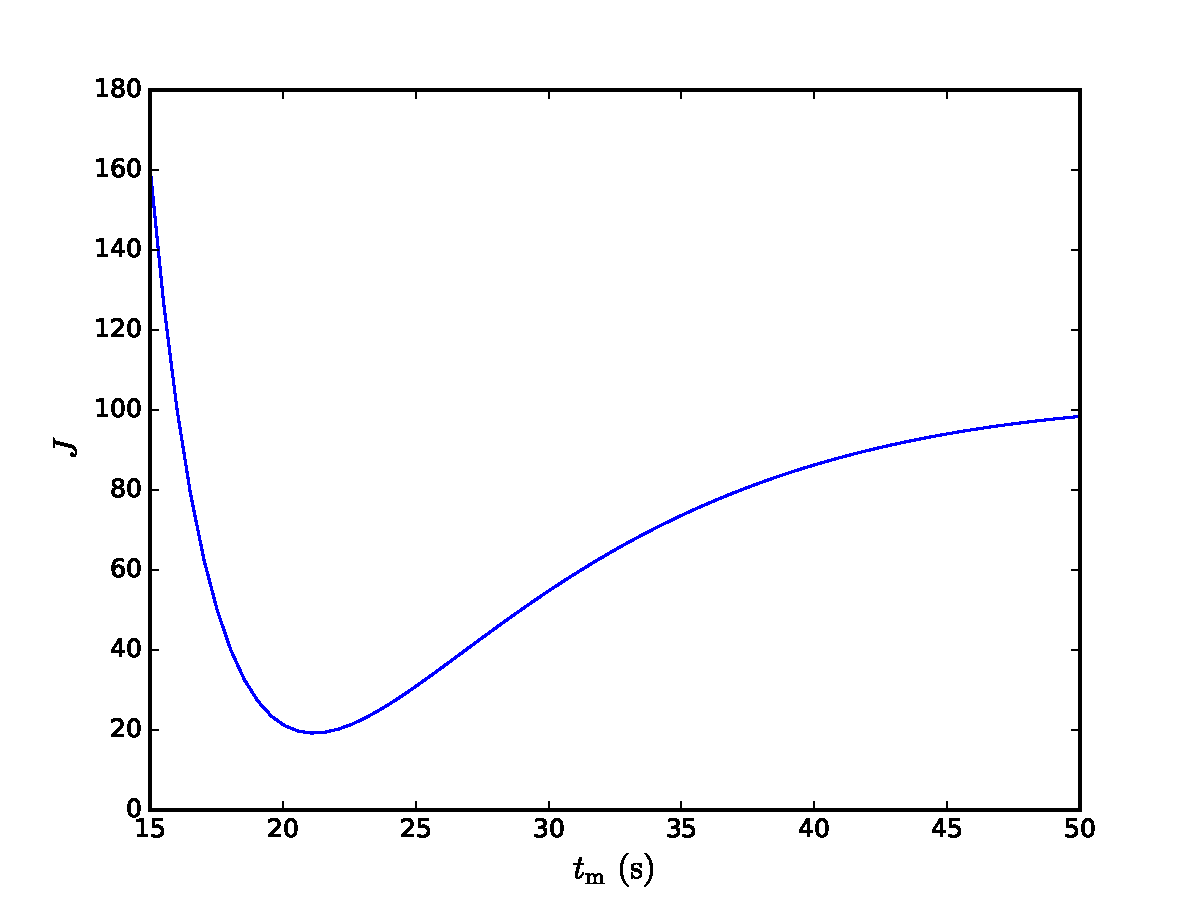
\includegraphics[width=10cm]{figures/tm.pdf}
\caption{$J\sim t_\mathrm{m}$关系曲线}
\label{fig:tm}
\end{figure}

图\ref{fig:tm}做出了$p_0=0$,$v_0=\SI{13.4}{m\per s}$,$L=\SI{400}{m}$,$v_\mathrm{m}=\SI{25.0}{m\per s}$条件下的$J\sim t_\mathrm{m}$关系曲线。经实验发现,在正常范围内,$J\sim t_\mathrm{m}$都是形如图\ref{fig:tm}的图线,很容易找到极小值。

\subsection{考虑控制量约束情形}
\label{ssec:c}
考虑速度、加速度的约束,某辆车的哈密尔顿函数为
\begin{multline}
H(p,v,u,t)=\frac12u^2+\lambda^\mathrm{p}v + \lambda^\mathrm{v}u+\\
\mu^\mathrm{a}(u-u_{\max})+\mu^\mathrm{b}(u_{\min}-u)+\mu^\mathrm{c}(v-v_{\max})+\mu^\mathrm{d}(v_{\min}-v),
\end{multline}
其中,$\mu^\mathrm{a},\mu^\mathrm{b},\mu^\mathrm{c}\mu^\mathrm{d}$为拉格朗日乘子,
\begin{align}
\mu^\mathrm{a}=\begin{dcases}
>0, & u(t)-u_{\max}=0,\\
=0, & u(t)-u_{\max}<0,
\end{dcases}\\
\mu^\mathrm{b}=\begin{dcases}
>0, & u_{\min}-u(t)=0,\\
=0, & u_{\min}-u(t)<0,
\end{dcases}\\
\mu^\mathrm{c}=\begin{dcases}
>0, & v(t)-v_{\max}=0,\\
=0, & v(t)-v_{\max}<0,
\end{dcases}\\
\mu^\mathrm{d}=\begin{dcases}
>0, & v_{\min}-v(t)=0,\\
=0, & v_{\min}-v(t)<0.
\end{dcases}
\end{align}
由伴随方程,
\begin{gather}
\lambda^\mathrm{p}=-\frac{\partial H}{\partial p} = 0,\\
\lambda^\mathrm{v}=-\frac{\partial H}{\partial v} =
\begin{dcases}
-\lambda^\mathrm{p}, & v(t)-v_{\max}<0 \quad \text{and}\\ & v_{\min}-v(t)<0,\\
-\lambda^\mathrm{p}-\mu^\mathrm{c}, & v(t)-v_{\max}=0,\\
-\lambda^\mathrm{p}+\mu^\mathrm{d}, & v_{\min}-v(t)=0.
\end{dcases}
\end{gather}
由控制方程,
\begin{equation}
\frac{\partial H}{\partial u}=u+\lambda^\mathrm{v}+\mu^\mathrm{a}-\mu^\mathrm{b}=0.
\end{equation}
下面根据是否触发约束条件分情况讨论。
\begin{enumerate}[label=(\arabic*)]
\item 未触发约束条件。这时哈密尔顿函数退化为\ref{ssec:noc}节所述的情形,因此最优控制为式\eqref{eq:ut}。
\item 触发约束条件,$u(t)=u_{\max}$且$v_{\min}<v(t)<v_{\max}$。假设在$t=t_1$时,该条件成立,则对于$\forall t>t_1$,
\begin{gather}
u^*(t)=u_{\max},\\
v^*(t)=u_{\max}t+f,\\
p^*(t)=\frac12u_{\max}t^2+ft+e.
\end{gather}
即车辆应按照最大加速度继续运行。其中参数$f$和$e$可由车辆在$t=t_1$时刻的位置和速度解出。
\item 触发约束条件,$u(t)=u_{\max}$且$v(t)=v_{\max}$,假设在$t=t_2>=t_1$时,$v(t)=v_{\max}$成立,则对于$\forall t>t_2$,
\begin{gather}
v^*(t)=v_{\max},\\
p^*(t)=v_{\max}t+q,\\
u^*(t)=\dot{v}^*(t)=0.
\end{gather}
车辆按照最大速度运行。其中参数$q$可由$t=t_2$时刻的位置解出。进一步地,如果在$t=t_3$时刻,车辆退出了该情况,即$v_{\min}<v(t)<v_{\max}$,则此时加速度应当重新回到线性形式,即
\begin{gather}
u^*(t)=gt+h,\label{eq:noc:lo1}\\
v^*(t)=\frac12gt^2+ht+r,\\
p^*(t)=\frac16gt^3+\frac12ht^2+rt+s.\label{eq:noc:lo3}
\end{gather}
其中参数$g$,$h$,$r$和$s$可仿照式\eqref{eq:noc:array}由该段初末状态解出。

\item 触发约束条件,$u(t)=u_{\min}$且$v_{\min}<v(t)<v_{\max}$。假设在$t=t_1$时,该条件成立,则对于$\forall t>t_1$,
\begin{gather}
u^*(t)=u_{\max},\\
v^*(t)=u_{\max}t+f,\\
p^*(t)=\frac12u_{\max}t^2+ft+e.
\end{gather}
即车辆应按照最大加速度减速运行。其中参数$f$和$e$可由车辆在$t=t_1$时刻的位置和速度解出。
\item 触发约束条件,$u(t)=u_{\min}$且$v(t)=v_{\min}$,假设在$t=t_2>=t_1$时,$v(t)=v_{\min}$成立,则对于$\forall t>t_2$,
\begin{gather}
v^*(t)=v_{\min},\\
p^*(t)=v_{\min}t+q,\\
u^*(t)=\dot{v}^*(t)=0.
\end{gather}
车辆按照最小速度运行。其中参数$q$可由$t=t_2$时刻的位置解出。进一步地,如果在$t=t_3$时刻,车辆退出了该情况,即$v_{\min}<v(t)<v_{\max}$,则此时加速度应当重新回到线性形式,最优控制由式\eqref{eq:noc:lo1}---\eqref{eq:noc:lo3}给出。
\item 触发约束条件,$v(t)=v_{\max}$且$u_{\min}<u(t)<u_{\max}$,假设在$t=t_2>=t_1$时,该条件成立,则对于$\forall t>t_2$,
\begin{gather}
v^*(t)=v_{\max},\\
p^*(t)=v_{\max}t+q,\\
u^*(t)=\dot{v}^*(t)=0.
\end{gather}
车辆按照最大速度运行。其中参数$q$可由$t=t_2$时刻的位置解出。进一步地,如果在$t=t_3$时刻,车辆退出了该情况,即$v_{\min}<v(t)<v_{\max}$,则此时加速度应当重新回到线性形式,最优控制由式\eqref{eq:noc:lo1}---\eqref{eq:noc:lo3}给出。
\item 触发约束条件,$v(t)=v_{\min}$且$u_{\min}<u(t)<u_{\max}$,假设在$t=t_2>=t_1$时,该条件成立,则对于$\forall t>t_2$,
\begin{gather}
v^*(t)=v_{\min},\\
p^*(t)=v_{\min}t+q,\\
u^*(t)=\dot{v}^*(t)=0.
\end{gather}
车辆按照最小速度运行。其中参数$q$可由$t=t_2$时刻的位置解出。进一步地,如果在$t=t_3$时刻,车辆退出了该情况,即$v_{\min}<v(t)<v_{\max}$,则此时加速度应当重新回到线性形式,最优控制由式\eqref{eq:noc:lo1}---\eqref{eq:noc:lo3}给出。
\end{enumerate}
\begin{remark}
对于以上讨论的触发约束的情况,按照约束值运行可以保证满足最优控制的必要条件。如果在某时刻退出了约束状态,只要后半段控制量为线性形式,仍然可以保证满足必要条件。由此可见,上述最优控制理论只给出了控制量的形式,至于某个控制序列是否为最优控制,还需要其他方式进行判断。下一章将要讨论的数值解法将会对此问题做出回答。
% \begin{enumerate}
% \item $t_i^c < t_{k} + \frac{\delta}{v_k^m}$, 按式(14),$t_i^{m*}=t_{k} + \frac{\delta}{v_k^m}$;
% \item 按照式(33)解最优控制发现超速,这时按下界走又会撞前车。此时应该怎样控制?
% \end{enumerate}
\end{remark}



%%% 其它部分

\backmatter

%% 本科生要这几个索引,研究生不要。选择性留下。
% 插图索引
\listoffigures
% 表格索引
\listoftables
% 公式索引
\listofequations


%% 参考文献
% 注意:至少需要引用一篇参考文献,否则下面两行可能引起编译错误。
% 如果不需要参考文献,请将下面两行删除或注释掉。
\bibliographystyle{thuthesis-numerical}
\bibliography{refs}


%% 致谢
% 如果使用声明扫描页,将可选参数指定为扫描后的 PDF 文件名,例如:
% \begin{acknowledgement}[scan-statement.pdf]
\begin{acknowledgement}
  衷心感谢导师 张毅 教授对本人的精心指导,与其博士生 封硕 师兄对我的帮助。他们的言传身教将使
  我终生受益。

  特拉华大学(University of Delaware)教授 Andreas Malikopoulos 的多篇文章给了我很大启发,并且详细解释了我对其论文的一些疑问,在此表示感谢。

  感谢我的父母和朋友在我毕设其间对我的帮助和支持。

  感谢 \thuthesis 项目及其维护者们,为我的毕业论文提供了格式和部分技术支持,大大减轻了我论文排版的工作量。
\end{acknowledgement}


%% 附录
\begin{appendix}
\chapter{外文资料原文}
\label{cha:engorg}

\title{The title of the English paper}

\textbf{Abstract:} As one of the most widely used techniques in operations
research, \emph{ mathematical programming} is defined as a means of maximizing a
quantity known as \emph{bjective function}, subject to a set of constraints
represented by equations and inequalities. Some known subtopics of mathematical
programming are linear programming, nonlinear programming, multiobjective
programming, goal programming, dynamic programming, and multilevel
programming$^{[1]}$.

It is impossible to cover in a single chapter every concept of mathematical
programming. This chapter introduces only the basic concepts and techniques of
mathematical programming such that readers gain an understanding of them
throughout the book$^{[2,3]}$.


\section{Single-Objective Programming}
The general form of single-objective programming (SOP) is written
as follows,
\begin{equation}\tag*{(123)} % 如果附录中的公式不想让它出现在公式索引中,那就请
                             % 用 \tag*{xxxx}
\left\{\begin{array}{l}
\max \,\,f(x)\\[0.1 cm]
\mbox{subject to:} \\ [0.1 cm]
\qquad g_j(x)\le 0,\quad j=1,2,\cdots,p
\end{array}\right.
\end{equation}
which maximizes a real-valued function $f$ of
$x=(x_1,x_2,\cdots,x_n)$ subject to a set of constraints.

\newtheorem{mpdef}{Definition}[chapter]
\begin{mpdef}
In SOP, we call $x$ a decision vector, and
$x_1,x_2,\cdots,x_n$ decision variables. The function
$f$ is called the objective function. The set
\begin{equation}\tag*{(456)} % 这里同理,其它不再一一指定。
S=\left\{x\in\Re^n\bigm|g_j(x)\le 0,\,j=1,2,\cdots,p\right\}
\end{equation}
is called the feasible set. An element $x$ in $S$ is called a
feasible solution.
\end{mpdef}

\newtheorem{mpdefop}[mpdef]{Definition}
\begin{mpdefop}
A feasible solution $x^*$ is called the optimal
solution of SOP if and only if
\begin{equation}
f(x^*)\ge f(x)
\end{equation}
for any feasible solution $x$.
\end{mpdefop}

One of the outstanding contributions to mathematical programming was known as
the Kuhn-Tucker conditions\ref{eq:ktc}. In order to introduce them, let us give
some definitions. An inequality constraint $g_j(x)\le 0$ is said to be active at
a point $x^*$ if $g_j(x^*)=0$. A point $x^*$ satisfying $g_j(x^*)\le 0$ is said
to be regular if the gradient vectors $\nabla g_j(x)$ of all active constraints
are linearly independent.

Let $x^*$ be a regular point of the constraints of SOP and assume that all the
functions $f(x)$ and $g_j(x),j=1,2,\cdots,p$ are differentiable. If $x^*$ is a
local optimal solution, then there exist Lagrange multipliers
$\lambda_j,j=1,2,\cdots,p$ such that the following Kuhn-Tucker conditions hold,
\begin{equation}
\label{eq:ktc}
\left\{\begin{array}{l}
    \nabla f(x^*)-\sum\limits_{j=1}^p\lambda_j\nabla g_j(x^*)=0\\[0.3cm]
    \lambda_jg_j(x^*)=0,\quad j=1,2,\cdots,p\\[0.2cm]
    \lambda_j\ge 0,\quad j=1,2,\cdots,p.
\end{array}\right.
\end{equation}
If all the functions $f(x)$ and $g_j(x),j=1,2,\cdots,p$ are convex and
differentiable, and the point $x^*$ satisfies the Kuhn-Tucker conditions
(\ref{eq:ktc}), then it has been proved that the point $x^*$ is a global optimal
solution of SOP.

\subsection{Linear Programming}
\label{sec:lp}

If the functions $f(x),g_j(x),j=1,2,\cdots,p$ are all linear, then SOP is called
a {\em linear programming}.

The feasible set of linear is always convex. A point $x$ is called an extreme
point of convex set $S$ if $x\in S$ and $x$ cannot be expressed as a convex
combination of two points in $S$. It has been shown that the optimal solution to
linear programming corresponds to an extreme point of its feasible set provided
that the feasible set $S$ is bounded. This fact is the basis of the {\em simplex
  algorithm} which was developed by Dantzig as a very efficient method for
solving linear programming.
\begin{table}[ht]
\centering
  \centering
  \caption*{Table~1\hskip1em This is an example for manually numbered table, which
    would not appear in the list of tables}
  \label{tab:badtabular2}
  \begin{tabular}[c]{|m{1.5cm}|c|c|c|c|c|c|}\hline
    \multicolumn{2}{|c|}{Network Topology} & \# of nodes &
    \multicolumn{3}{c|}{\# of clients} & Server \\\hline
    GT-ITM & Waxman Transit-Stub & 600 &
    \multirow{2}{2em}{2\%}&
    \multirow{2}{2em}{10\%}&
    \multirow{2}{2em}{50\%}&
    \multirow{2}{1.2in}{Max. Connectivity}\\\cline{1-3}
    \multicolumn{2}{|c|}{Inet-2.1} & 6000 & & & &\\\hline
    \multirow{2}{1.5cm}{Xue} & Rui  & Ni &\multicolumn{4}{c|}{\multirow{2}*{\thuthesis}}\\\cline{2-3}
    & \multicolumn{2}{c|}{ABCDEF} &\multicolumn{4}{c|}{} \\\hline
\end{tabular}
\end{table}

Roughly speaking, the simplex algorithm examines only the extreme points of the
feasible set, rather than all feasible points. At first, the simplex algorithm
selects an extreme point as the initial point. The successive extreme point is
selected so as to improve the objective function value. The procedure is
repeated until no improvement in objective function value can be made. The last
extreme point is the optimal solution.

\subsection{Nonlinear Programming}

If at least one of the functions $f(x),g_j(x),j=1,2,\cdots,p$ is nonlinear, then
SOP is called a {\em nonlinear programming}.

A large number of classical optimization methods have been developed to treat
special-structural nonlinear programming based on the mathematical theory
concerned with analyzing the structure of problems.
\begin{figure}[h]
  \centering
  \includegraphics{thu-lib-logo}
  \caption*{Figure~1\quad This is an example for manually numbered figure,
    which would not appear in the list of figures}
  \label{tab:badfigure2}
\end{figure}

Now we consider a nonlinear programming which is confronted solely with
maximizing a real-valued function with domain $\Re^n$.  Whether derivatives are
available or not, the usual strategy is first to select a point in $\Re^n$ which
is thought to be the most likely place where the maximum exists. If there is no
information available on which to base such a selection, a point is chosen at
random. From this first point an attempt is made to construct a sequence of
points, each of which yields an improved objective function value over its
predecessor. The next point to be added to the sequence is chosen by analyzing
the behavior of the function at the previous points. This construction continues
until some termination criterion is met. Methods based upon this strategy are
called {\em ascent methods}, which can be classified as {\em direct methods},
{\em gradient methods}, and {\em Hessian methods} according to the information
about the behavior of objective function $f$. Direct methods require only that
the function can be evaluated at each point. Gradient methods require the
evaluation of first derivatives of $f$. Hessian methods require the evaluation
of second derivatives. In fact, there is no superior method for all
problems. The efficiency of a method is very much dependent upon the objective
function.

\subsection{Integer Programming}

{\em Integer programming} is a special mathematical programming in which all of
the variables are assumed to be only integer values. When there are not only
integer variables but also conventional continuous variables, we call it {\em
  mixed integer programming}. If all the variables are assumed either 0 or 1,
then the problem is termed a {\em zero-one programming}. Although integer
programming can be solved by an {\em exhaustive enumeration} theoretically, it
is impractical to solve realistically sized integer programming problems. The
most successful algorithm so far found to solve integer programming is called
the {\em branch-and-bound enumeration} developed by Balas (1965) and Dakin
(1965). The other technique to integer programming is the {\em cutting plane
  method} developed by Gomory (1959).

\hfill\textit{Uncertain Programming\/}\quad(\textsl{BaoDing Liu, 2006.2})

\section*{References}
\noindent{\itshape NOTE: These references are only for demonstration. They are
  not real citations in the original text.}

\begin{translationbib}
\item Donald E. Knuth. The \TeX book. Addison-Wesley, 1984. ISBN: 0-201-13448-9
\item Paul W. Abrahams, Karl Berry and Kathryn A. Hargreaves. \TeX\ for the
  Impatient. Addison-Wesley, 1990. ISBN: 0-201-51375-7
\item David Salomon. The advanced \TeX book.  New York : Springer, 1995. ISBN:0-387-94556-3
\end{translationbib}

\chapter{外文资料的调研阅读报告或书面翻译}

\title{城市道路自动驾驶车辆运动计划和控制研究综述}

{\heiti 摘要:} 自动驾驶车是一种成熟的技术,通过提高汽车运输的安全性,可及性,效率和便利性,有可能重塑人们的出行方式。 自驾车必须在确保安全的前提下执行任务,包括通过与其他车辆和行人共享的动态环境进行动作规划,以及通过反馈控制可靠地执行动作。 本文的目的是调查目前的规划和控制算法的现状,特别是在城市环境中。本文对部分所提出的技术进行了综述,并讨论了其有效性。 所调查的方法在所使用的车辆移动性模型,环境结构假设和计算要求方面不同。 本次调查中的并列比较有助于深入了解经过调查的方法的优势和局限性,并辅助系统级设计选择。

\section{介绍}

过去三十年来,学术界和工业界都在不断开展无人驾驶技术的研究工作。传感和计算技术的最新进展,无人驾驶技术对汽车运输的潜在转变及其社会效益,推动了这项技术的发展:2014年有交通相关死亡人员32,675人,其中230万人受伤,610万起交通事故被报道[1]。其中,估计有94\%的事故是由驾驶员操作失误造成,31\%涉及饮酒的驾驶员,10\%涉及分心的驾驶员[2]。自动驾驶车有可能大大减少因驾驶员犯错和疏忽而造成的事故。它们还将为由于身体或视觉残疾而无法驾驶的人提供私人交通工具。最后,全美工作人口86\%的人每天平均花25分钟(单程)的时间乘汽车上下班,自动驾驶车将有助于更有效地利用通勤时间,或简单地减少驾驶压力带来的不良影响[4]。

考虑到这种新技术的潜在影响,自驾车已经有悠久的历史。这个想法早在20世纪20年代就已经存在,但直到20世纪80年代,无人驾驶的汽车才真正成为可能。 20世纪80年代由恩斯特·迪克曼(Ernst Dickmanns)(例如[5])领导的开创性工作为无人车的开发铺平了道路。那时候,PROMETHEUS项目的大量研究力量投入了无人车的研发。 1994年,由VaMP开发的无人驾驶汽车驾驶1600公里,其中95\%是自主驾驶[6]。在同一时期,CMU NAVLAB正在该领域取得进展,并在1995年展示了进一步的进展,在5000公里穿越美国的车程中,98\%是自主驾驶[7]。

无人驾驶汽车技术的下一个重大里程碑是2004年第一次DARPA大挑战赛。比赛目标是让无人驾驶汽车尽快通过150英里的越野赛道。与以前的展示相比,这是一个重大的挑战,因为在比赛中不会有人为的干预。虽然以前的工作能实现几乎自主的驾驶,但在关键时刻消除人为干预被证明是一个重大的挑战。15辆车中没有一辆完成比赛。 2005年举办了类似的活动;这一次,23支队伍中有5个到达了终点线[8]。后来,2007年,DARPA城市挑战赛举行,车辆被要求在模拟城市环境中自主驾驶。六个小组完成了这一比赛,表明完全自主的城市驾驶是可能的[9]。

自从DARPA挑战以来,全世界已经进行了许多比赛和较大的无人车系统测试。值得注意的例子包括2009年至2013年的智能车辆未来挑战赛[10],2010年的现代汽车无人车挑战赛[11],2010年的VisLab洲际无人车挑战赛[12],2013年的城市无人驾驶汽车公路测试[13],以及Bertha-Benz路线的自主驾驶测试[14]。同时,在学术环境的改善和行业发展的驱动下,无人车研究工作进展顺利。 Google自驾车[15]和特斯拉的自动驾驶仪系统[16]是获得广泛关注的商业活动的两个例子。

汽车自动化的程度可以从完全由人操作到完全自主操作。 SAE J3016标准[17]引入了从0到5的等级分级车辆自动化程度。在这个标准中,0级代表车辆所有驾驶任务都是人类驾驶员完成。1级包括基本驾驶辅助,如自适应巡航控制,防抱死制动系统和电子稳定控制[18]。2级包括高级辅助系统,如危害最小化纵向/横向控制[19]和紧急制动[20],[21],这些系统通常基于预先设定形式的控制理论来计算“最坏情况” (安全)状态[22] - [24],确保车辆无碰撞。在3级系统中,系统对行车环境进行监控,并且可以在某些条件下完全自主地运行,但如果驾驶任务离开自主系统的操作范围,则仍然需要操作人员进行控制。具有4级自动化的车辆能够在某些条件下完全自主驾驶,并且如果操作者没有根据要求进行干预,仍可以安全地控制车辆。 5级系统在所有驾驶模式下都是完全自主的。

车载计算和无线通信技术的可用性允许汽车与其他车辆和道路基础设施交换信息,引发了与之密切相关的智能网联车技术的研究[25]。这方面研究旨在通过个别车辆之间的信息共享和协调来提高道路运输的安全性和性能。例如,网联车技术有可能改善交叉点处的吞吐量[26]或阻止交通冲击波的形成[27]。

为了限制本次调查的范围,我们专注于自主驾驶汽车的决策,运动规划和控制方面,特别是对于3级及以上的自动化系统。出于同样的原因,自动驾驶车的感知技术被忽略,读者可以参考关于这一主题的一些综述和近期的重要进展[28] - [31]。

当代自主驾驶系统的决策通常分层次地组织成路线规划,行为决策,局部运动规划和反馈控制。然而,文献中有许多不同的划分,因此对决策级别的划分相当模糊。本文对于解决这些自主驾驶核心问题所提出的方法展开了调查,特别强调局部运动规划和控制的方法。

本文的其余部分结构如下:第二部分对决策过程层次进行了概述,展示了部分设计方法。第三节回顾了用于在城市环境中估计汽车的移动性的模型,以便进行运动规划和反馈控制的研究。第四节调查有关运动规划的丰富文献,并讨论其对自驾车的适用性。同样,第五节讨论了无人驾驶汽车的路径和轨迹稳定问题以及具体的反馈控制方法。最后,第六部分总结了并评述了研究现状和未来研究方向。


\section{无人车决策层次概述}

在本节中,我们将描述典型自驾车的决策层次,并对每个部分的功能进行描述。无人驾驶汽车本质上是自动决策系统,可处理来自车载传感器(如雷达,LIDAR,摄像机,GPS / INS单元和测距仪)的观测数据流。这些观察结果以及关于道路网络的现有知识,道路规则,车辆动力学和传感器模型被用于自动选择控制车辆运动的控制变量的值。智能车辆研究旨在尽可能多地自动化驾驶任务。该问题通常采用的方法是将感知和决策任务分解和组织成一个层次结构。感知系统使用先前的信息和收集的观测数据来提供车辆状态及对周围环境的估计,然后由决策系统使用估计来控制车辆,从而完成驾驶目标。

典型自驾车的决策系统被分层分解为四个组成部分(参见图\ref{fig:decision}):在最高层,路线是通过道路网计划的。这之后是一个行为层,决定了一个局部的驾驶任务,逐渐将汽车导向目的地,并兼顾交通规则。运动规划模块然后在通行环境中规划一条连续路径以完成局部导航任务。最后由控制系统在运动的执行中反馈性地纠正错误。在本节的其余部分,我们将更详细地讨论每个部分的功能。

\begin{figure}
\centering
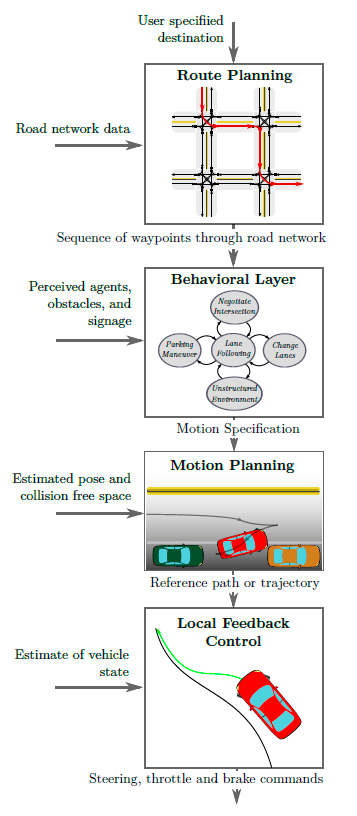
\includegraphics[width=8cm]{decision.png}
\caption{无人车决策层级图}
\caption*{目的地作为路径规划层的输入,生成路网上的路径。行为决策层根据该路径和周围环境,生成一列指向目的地的具体行动。运动规划层进而规划出完成该行动的可行路径。反馈控制调整执行变量以纠正执行参考路径中的错误。}
\label{fig:decision}
\end{figure}

\subsection{路径规划}
在最高级别,车辆的决策系统必须选择通过道路网从当前位置到所要求的目的地的路线。通过将道路网络表示为具有与穿越该路段的成本相对应的赋权有向图,可以将路径规划问题转化为在道路网络图上找到最小成本路径的问题。然而,代表道路网络的图形可以包含数百万条边,使得经典的最短路径算法(如Dijkstra [32]或A * [33])不切实际。运输网络中高效路线规划的问题引起了运输科学界的极大兴趣,研究者发明了一系列算法,经过一次性预处理步骤,可以在几毫秒内在大陆规模的网络上返回最佳路径[34],[35]。对于可用于有效规划驾驶员驾驶和自动驾驶车路线的实际算法的综合调查和比较,参见[36]。

\subsection{行为决策}
在找到路线之后,无人车必须能够根据交通规则,导航所选择的路线,并与其他交通参与者进行交互。给定指示所选路线的路段的序列,行为决策层负责根据其他交通参与者的感知行为,路况和基础设施的信号在任意时间点选择合适的驾驶行为。例如,当车辆在交叉口前到达停车线时,行为层将命令车辆停下来,观察交叉路口处的其他车辆,自行车和行人的行为,并当轮到本车运行时发出运行指令。驾驶手册规定了具体驾驶环境的定性动作。由于驾驶环境和每个环境中可用的行为都可以被建模为有限集,自动化这种决策的自然方法是将每个行为建模成有限状态机中的状态,其中转移由感知到的驾驶环境控制,如本车相对于计划路线和附近车辆的位置。事实上,DARPA城市挑战中大多数团队都采用了有限状态机与特定于驾驶场景的不同启发式搜索[9]作为行为控制机制。

然而,现实世界的驾驶,特别是在城市中,其他交通参与者的意图不确定。研究者们还研究了其他车辆,自行车和行人未来轨迹的意图预测和估计问题。所提出的解决方案是基于机器学习的技术,例如高斯混合模型[37],高斯过程回归[38](这种方法被用于Google自主驾驶系统中意图预测的学习[39]),以及基于模型的直接从传感器测量数据估计意图的方法[40],[41]。

其他交通参与者的行为中的这种不确定性在行为决策层中通常建模为概率模型(例如马尔可夫决策过程(MDP))。例如,[42]在MDP框架中制定行为决策。一些工作[43] - [46]将未观察到的驾驶场景和行人意图显式建模为部分可观察的马尔可夫决策过程(POMDP),并提出具体的求近似解的策略。

\subsection{运动规划}
当行为层决定在当前环境中执行的驾驶行为,例如跟驰,换道或右转时,所选择的行为必须被转换为路径或轨迹,才可以由低级反馈控制器跟踪。所得到的路径或轨迹必须对于车辆而言是动态可行的,对于乘客来说舒适,并且避免与车载传感器检测到的障碍物的碰撞。找到这样的路径或轨迹是运动规划系统的任务。

无人车的运动规划任务与机器人控制相关文献中讨论的求解标准运动规划的问题密切相关。在大多数情况下,运动规划问题的精确解决方案在计算上是不可行的。因此,在实践中通常使用数值近似方法。最常用的数值方法有变分法、图搜索发和增量树法等。其中变分法将轨迹求解问题转化为函数空间中的非线性优化问题;图搜索方法将构成车辆状态空间的道路拓扑图离散化并搜索最短路径;增量树法从车辆的初始状态逐渐构建可达状态树,然后选择这样一棵树的最佳分支。自动驾驶相关的运动规划方法在第四节中有更详细的讨论。

\subsection{车辆控制}
为了执行运动规划系统确定的参考路径或轨迹,无人车使用反馈控制器来选择适当的执行器输入以执行计划的运动和纠正跟踪误差。 执行计划运动期间产生的跟踪误差部分原因在于车辆模型的不准确。 因此,闭环系统的鲁棒性和稳定性非常重要。

研究者们已经设计了许多有效的反馈控制器,来执行由运动规划系统提供的参考路径或轨迹。 相关技术在第五节中有详细的讨论。

\section{无人车运动模型}
在本节中,我们将调查最常用的车辆运动模型。这些模型被广泛用于控制和运动规划算法中,来近似车辆的行为,响应相关操作条件下的控制动作。高保真模型可以准确反映车辆对控制量输入的响应,但是附加的细节可能使计划和控制问题复杂化。这提供了所选模型的准确性与决策问题的难度之间的权衡。本节概述了一般建模概念和运动规划和控制模型。

建模从车辆配置的概念开始,代表其在世界上的姿势或位置。例如,配置可以表示为汽车上的点与汽车的航向的平面坐标。这是汽车配置空间的坐标系。该坐标系描述平面刚体运动(由特殊欧几里德组在两维中表示,SE(2)),并且是常用的配置空间[47] - [49]。车辆运动的规划和调整必须在遵循所选模型引入的限制的前提下,完成驾驶任务。

\subsection{单轨道运动学模型}
在实际使用的最基本模型中,汽车由两个通过刚性连杆连接的轮子组成,并被限制在一个平面上移动[48] - [52]。 假设车轮在与地面的接触点处不会滑动,而可以绕其旋转轴线自由旋转。 前轮具有附加的自由度,允许其绕垂直于运动平面的轴线旋转,以对转向进行建模。 该模型的这两个特征反映了大多数乘客在不同时前进的情况下不能进行横向位移的经验。 更正式地说,这种机动性的限制被称为非完整约束[47],[53]。 非完整约束被表示为对汽车运动的差分约束。 该表达式取决于坐标系的选择。 该模型的各种变种通常被称为类车机器人,自行车模型,运动模型或单轨道模型。

以下是用于配置的几个常用坐标系中差分约束的推导。 参考图\ref{fig:kinematics},矢量$p_r$和$p_f$表示后轮和前轮在具有基矢量$(\hat{e}_x, \hat{e}_y, \hat{e}_z)$的静止或惯性坐标系中的位置。朝向角$\theta$是描述车辆所面向的方向的角度,定义为向量$\hat{e}_x$和$p_f-p_r$之间的角度。
\begin{figure}
\centering
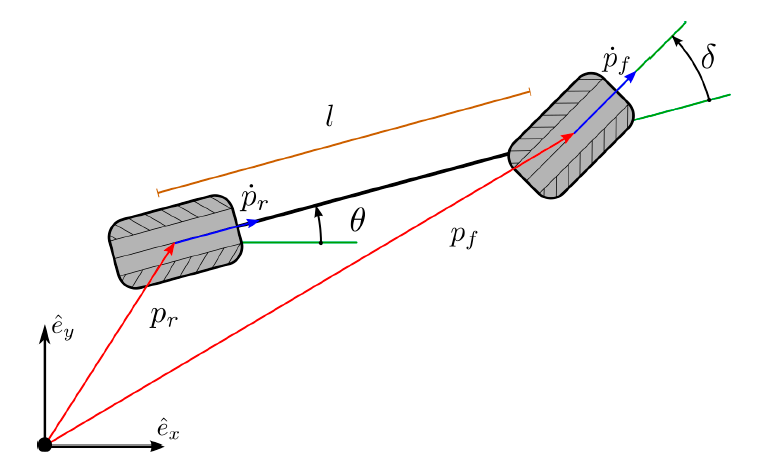
\includegraphics[width=13cm]{kinematics.png}
\caption{单轨道运动学模型图}
\caption*{$p_r$与$p_f$分别为后轮、前轮与地面的触点,$\theta$是车辆朝向角。$p_r$与$p_f$对时间的导数的方向受到非完整性约束的限制,如图中蓝色箭头所示。$\delta$是前轮导向角。}
\label{fig:kinematics}
\end{figure}

下面将对于包含朝向角$\theta$,点$p_r$的运动,点$p_f$的运动的坐标系导出差分约束。

为了满足接触点不滑动的约束,点$p_r$,$p_f$的运动必须与轮子的朝向共线,对后轮,该约束表示为
\begin{equation}
(\dot{p}_r\cdot \hat{e}_y)\cos(\theta)-(\dot{p}_r\cdot \hat{e}_x)\sin(\theta)=0,
\end{equation}
对前轮,有
\begin{equation}
(\dot{p}_f\cdot \hat{e}_y)\cos(\theta+\delta)-(\dot{p}_f\cdot \hat{e}_x)\sin(\theta+\delta)=0.
\end{equation}
该表达式通常被重写为关于基向量的分量形式。后轮运动在$\hat{e}_x$方向的分量为$x_r := p_r\cdot\hat{e}_x$,在$\hat{e}_y$方向为$y_r:=p_r\cdot \hat{e}_y$。前进速度为$v_r:=\dot{p}_r\cdot(p_f-p_r)/\|(p_f-p_r)\|$,即$\dot{p}_r$的模长乘上表示方向的符号。关于标量$x_r$,$y_r$和$\theta$,差分约束表示为
\begin{align}
\begin{split}
\dot{x}_r&= v_r\cos(\theta),\\
\dot{y}_r&= v_r\sin(\theta),\\
\dot{\theta}&=\frac{v_r}{l}\tan(\delta).
\end{split}
\end{align}
同样,对于点$p_f$的运动也具有差分约束
\begin{align}
\begin{split}
\dot{x}_f&= v_f\cos(\theta),\\
\dot{y}_f&= v_f\sin(\theta),\\
\dot{\theta}&=\frac{v_f}{l}\tan(\delta).
\end{split}
\label{eq:vf}
\end{align}
其中,前轮速度$v_f$与后轮速度有关系
\begin{equation}
\frac{v_r}{v_f}=\cos(\delta).
\end{equation}

对该车辆模型的规划和控制需要决定前轮导向角$\delta\in [\delta_{\min}, \delta_{\max}]$和前进速度$v_r\in [v_{\min}, v_{\max}]$。

一个常用的简化,如在[56]中用到的,是选择航向率$\omega$,而不是导向角$\delta$。二者存在关系
\begin{equation}
\delta=\arctan(\frac{l\omega}{v_r})
\end{equation}
这将朝向的运动简化为
\begin{equation}
\dot{\theta}=\omega, \quad \omega\in [\frac{v_r}{l}\tan(\delta_{\min}, \frac{v_r}{l}\tan(\delta_{\max})]
\end{equation}
这种模型有时被称为单轮车模型,因为它可以通过考虑单个车轮的运动而得出。

单轨道运动模型的一个重要变种是固定$v_r$的情况。 这有时被称为杜宾斯车,以莱斯特·杜宾斯(Lester Dubins)命名,他在规定切线的情形下得出了两点之间的最短时间运动[57]。另一个重要变种是Reed-Shepp车,当$v_r$取单值的正向和反向速度时,可以求出最小长度的路径[58]。 这两个模型已被证明对运动规划具有重要意义,并将在第四节进一步讨论。

运动学模型适用于低速情形,例如停车机动和城市驾驶。在该情形下车的惯性较小,不足以打破车轮不打滑的假设。该模型的主要缺点是它允许转向角度瞬间变化。如果运动计划模块要求产生这种瞬时变化,这将是有问题的。

转向角的连续性可以通过改进(\ref{eq:vf})来实现,其中转向角是转角速率的积分,如[49]所示。 方程式(\ref{eq:vf})变为
\begin{align}
\begin{split}
\dot{x}_f&= v_f\cos(\theta),\\
\dot{y}_f&= v_f\sin(\theta),\\
\dot{\theta}&=\frac{v_f}{l}\tan(\delta),\\
\dot{\delta}&=v_{\delta}.
\end{split}
\end{align}
除了对导向角的连续性限制,转角变化率也可以引入约束$v_{\delta}\in [\dot{\delta}_{\min},\dot{\delta}_{\max}]$。同样的问题也会出现在速度控制上。可以通过引入加速度保证速度控制的连续性。这种方法的缺点在于增加了模型的维数,将运动计划与控制问题变得更为复杂。

坐标系的选择不限于使用一个车轮位置作为位置坐标。 对于使用经典力学原理得出的模型,可以使用质心作为位置坐标,如[59],[60]或使用振荡中心,如[61],[62]。

\chapter{其它附录}
前面两个附录主要是给本科生做例子。其它附录的内容可以放到这里,当然如果你愿意,可
以把这部分也放到独立的文件中,然后将其 \cs{input} 到主文件中。

\end{appendix}

%% 个人简历
\include{data/resume}

%% 本科生进行格式审查是需要下面这个表格,答辩可能不需要。选择性留下。
% 综合论文训练记录表
\includepdf[pages=-]{scan-record.pdf}
\end{document}